\section{Grundlagen \textit{KNNs} \& \textit{DNN}s}

In diesem Kapitel werden die theoretischen Grundlagen für die in dieser Arbeit verwendeten Algorithmen behandelt. In einer Einleitung werden die Begrifflichkeiten erläutert sowie die Motivation wie auch Schwierigkeiten für die Entwicklung von \textit{maschinellen Lernalgorithmen} (\textit{ML}) geschildert. Der Hauptteil behandelt den technischen Aspekt von \textit{KNN}s und \textit{DNN}s, worin das Funktionsprinzip, verschiedene Architekturen als auch Umsetzungstechniken vorgestellt werden.

Es ist anzumerken, dass es sich bei \textit{maschinellem Lernen} und \textit{künstlichen neuronalen Netzen} um ein sehr komplexes Themengebiet handelt. Für das Verständnis des Theorieteils wird somit ein solides Grundwissen für technische als auch mathematische Konzepte vorausgesetzt, um die relevanten Informationen in einem angemessenen Umfang behandeln zu können.

\subsection{\textit{KI}, \textit{KNN}, \textit{DL}, usw.}
In den Medien wie auch im Internet hört und liest man die Ausdrücke und Abkürzungen immer wieder: \textit{KI}s, \textit{Deep Learning} und \textit{neuronale Netze}, \textit{AI}s und \textit{DNN}s. Man könnte meinen, sie seien ähnlich, jedoch bedeuten sie nicht alle dasselbe. Folgender Überblick soll helfen, die verwirrenden Bezeichnungen und Fachausdrücke korrekt zu interpretieren. Der Inhalt greift dabei etwas vor, um späteres Nachschlagen zu ermöglichen.

\begin{itemize}[leftmargin=2cm]
	\item[\textbf{\textit{KI}}:] Künstliche Intelligenz \textit{(engl. artificial intelligince, AI)}:\\
	 Überbegriff in der Informatik für automatisierte Prozesse, welche ''intelligentes'' Verhalten modellieren/nachahmen. Mangels einer klaren Definition von ''Intelligenz'' ist der Begriff sehr weit anwendbar\cite{ai}, d.h. einen Roboter auf zwei Beinen gehen zu lassen gehört genau so zur \textit{KI} wie die Erkennung von Gesichtern.
	 
	\item[\textbf{\textit{ML}}:] Maschinelles Lernen \textit{(engl. machine learning)}:\\
	Teilbereich der \textit{künstlichen Intelligenzen}, welcher sich mit künstlichen Lernprozessen befasst. Konventionellen Programmen gibt man einen Satz an Regeln mit, um z.B. Muster erkennen zu können. Beim \textit{maschinellen Lernen} ist es hingegen das Ziel, den Algorithmus durch Training die Regeln und Gesetzmässigkeiten selber erkennen und bestimmen zu lassen. Für den Trainingsprozess werden meistens bezeichnete Trainingsdaten verwendet\cite{ml}. 
	
	\item[\textbf{\textit{KNN/NN}}:] Künstliches neuronales Netz \textit{(engl. artificial neural network, ANN)}:\\
	Programmtechnik aus dem Gebiet des \textit{maschinellen Lernens}, welche inspiriert biologischen neuronalen Netzen (Gehirnen) Neuronen und deren Interaktionen zu modellieren versucht. Die \textit{Neuronen} sind in Schichten angeordnet (sog. \textit{Layers}) und untereinander verbunden. \textit{KNN}s sind in der Lage aus Trainingsdaten zu lernen\cite{ann}. Im Kontext der Informatik wird zwischen \textit{künstlichen neuronalen Netzen} und \textit{neuronalen Netzen} (\textit{NN}s) nicht differenziert.
	
	\item[\textbf{\textit{SNN}}:] Shallow Neural Network:\\
	Eher selten gebrauchter Begriff, \textit{KNN} impliziert z.T. ein \textit{SNN}\footnote{Um Missverständnisse zu meiden, werden in dieser Arbeit die Begriffe \textit{KNN} und \textit{NN} als \textbf{Überbegriff} von \textit{SNN}s und \textit{DNN}s verwendet.}. ''Shallow'' weist dabei auf die geringe Anzahl der \textit{Layers} hin (i.d.R. 1, höchstens 2 \textit{Hidden Layers}). Wegen den wenigen \textit{Layers} können \textit{SNN}s nur einfachere Probleme lösen\cite{ann}.
		
	\item[\textbf{\textit{DL/DNN}}:] Deep Learning/Deep Neural Network:
	Im Gegensatz zu \textit{SNN}s bezeichnet man mit \textit{Deep Learning} Netzarchitekturen, welche 2 oder mehr \textit{Hidden Layers} besitzen. Mit speziellen \textit{Layers} können dem \textit{KNN} andere Eigenschaften oder Charakteristiken gegeben werden, so z.B. verbesserte Verallgemeinerung oder ein ''Kurzzeitgedächtnis''. \textit{Deep Neural Network} weist spezifisch auf die Umsetzung eines \textit{DL}-Algorithmus mit \textit{NN}s hin, jedoch werden die beiden Begriffe meist synonym verwendet\cite{dl}.
	
	\item[\textbf{\textit{CNN}}:] Convolutional Neural Network:\\
	 Spezielle Art eines \textit{Deep Neural Networks}, welche sich v.a. in der Bilderkennung bewährt. Mit verschiedenen \textit{Layers} werden die relevanten Informationen gefiltert und auf immer kleinere \textit{Layers} konzentriert. Diese Massnahme ermöglicht sehr komplexe und leistungsfähige Netze in absehbarer Zeit zu trainieren.
	
\end{itemize}

\newpage

\subsection{Einleitung}


\begin{figure}[h]
	\centering
	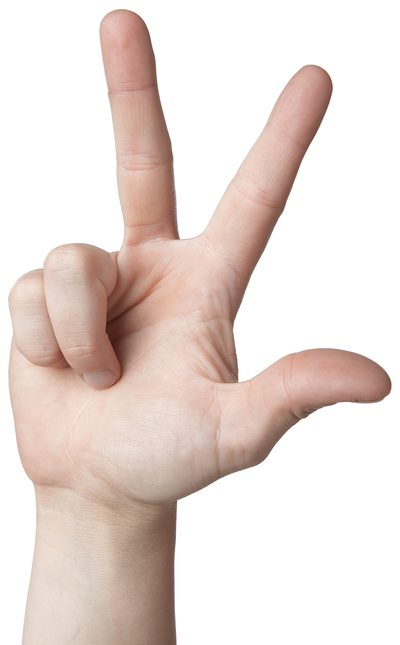
\includegraphics[width= 3cm]{fingers}
	\caption[Finger, https://img.livestrongcdn.com/, 2017, Artikel 541001]{Finger}
\end{figure}

Sie haben wahrscheinlich ohne zu zögern das Bild gesehen und sofort erkannt, dass darauf eine Hand mit 3 ausgestreckten Fingen gezeigt wird. Es scheint auf den ersten Blick ein simpler Prozess zu sein. So simpel, dass sogar Kleinkinder dazu fähig sind. Mit dieser Vorstellung waren ersten \textit{KI}-Forscher der 1960er der Meinung, sie könnten Rechnern die visuellen Interpretation von Bildern wie auch andere menschliche Fähigkeiten beibringen --- in der Zeitspanne von nur zwanzig Jahren. Wie es sich herausstellte, haben sie die Hürde massiv unterschätzt. Erst heute mit der steigenden Rechenleistung und neuen Entwicklungen beginnen die Computer langsam die Versprechen der 60er zu erfüllen. In anderen Worten: Ihr visueller Kortex hat für die Erkennung dieser Finger soeben das geleistet, wofür Rechner Jahrzehnte an Forschung und Entwicklung benötigt haben.\\


\epigraph{\setstretch{2}{\Large ''Maschinen werden in 20 Jahren zu jeder Arbeit fähig sein, die ein Mensch verrichten kann.''}\cite{hasimon}}{\textit{Herbert A. Simon\\ \textit{KI}-Pionier, 1965}}

Um die Schwierigkeiten der Bilderkennung zu verstehen, muss das Problem aus der sich von Rechnern betrachtet werden. Was wir als ein Bild von einer Hand erkennen sind für einen Computer Zahlen. Jeder Bildpunkt (\textit{Pixel}) besteht aus drei Intensitätswerten zwischen 0 und 255 für die Grundfarben rot, grün und blau; im Raster angeordnet ergeben sie das Bild. Die Frage besteht in diesem Beispiel darin, ob eine mathematische Funktion\footnote{Laut Alan Turing kann jede mathematische Funktion als Computerprogramm umgesetzt werden\cite{alanturing}, weswegen das Finden dieser Funktion das eigentliche Ziel ist.} für diese Pixelwerte gefunden werden kann, welche etwas über die Anzahl der gezeigten Finger aussagen kann. In Worten formuliert sähe die Funktion wie folgt aus: ''Ein ausgestreckter Finger ist leicht rötlich, länglich und von der Hand gespreizt. Diese gilt es zu zählen''. Will man nun aber einen Algorithmus designen, welche diese Eigenschaften erkennen kann, so verliert man sich schnell in unzähligen Regeln und komplexen Ausnahmen. Es sei denn, man lässt den Algorithmus anhand von Beispieldaten die Muster und Regeln selber finden:

\subsection{Maschinelles Lernen}\label{cha:theo:ml}
Maschinelle Lernalgorithmen sind auf den künstlichen Wissenserwerb spezialisiert. Dabei ist es wichtig, nicht durch ''Auswendiglernen'', sondern durch Erkennen und Verallgemeinern von Gesetzmässigkeiten Daten zu verarbeiten. Es sind viele verschiedene Umsetzungsansätze für lernfähige Algorithmen bekannt; so z.B. \textit{genetische Algorithmen}, \textit{Entscheidungsbäume} und \textit{künstliche neuronale Netze}.

\paragraph{Training} Um ''Wissen zu erwerben'' werden maschinelle Lernalgorithmen \textit{trainiert}. Der \textit{Trainingsprozess} sieht generell folgendermassen aus: Ein Datensatz aus den \textit{Trainingsdaten} wird in den zu trainierenden Algorithmus eingespeist, worauf das erhaltene (meist falsche) Ergebnis mit dem erwünschten Ergebnis verglichen wird. Durch Anpassung der \textit{Parameter} des Algorithmus wird versucht, das Resultat zu verbessern. Dieser Prozess wird mit allen Datensätzen der Trainingsdaten wiederholt, wodurch der Algorithmus eine allgemein anwendbare Funktion für die Zuordnung von Eingangsdaten zum korrekten Ergebnis finden soll.

\subsubsection{Verzerrung-Varianz-Dilemma \cite{bias}}\label{cha:theo:ml:b-v}
Das Verzerrung-Varianz-Dilemma ist eine generelle Schwierigkeit von Lernalgorithmen. Der Algorithmus soll mit den \textit{Trainingsdaten} als auch mit komplett neuen Daten akkurate Ergebnisse liefern können.

Nehmen wir uns folgendes vereinfachtes Beispiel vor: Von einer unbekannten Funktion $f(x)$ sind einige Datenpunkte bekannt, welche als Trainingsdaten verwendet werden sollen:

\begin{figure}[h]
	\centering
	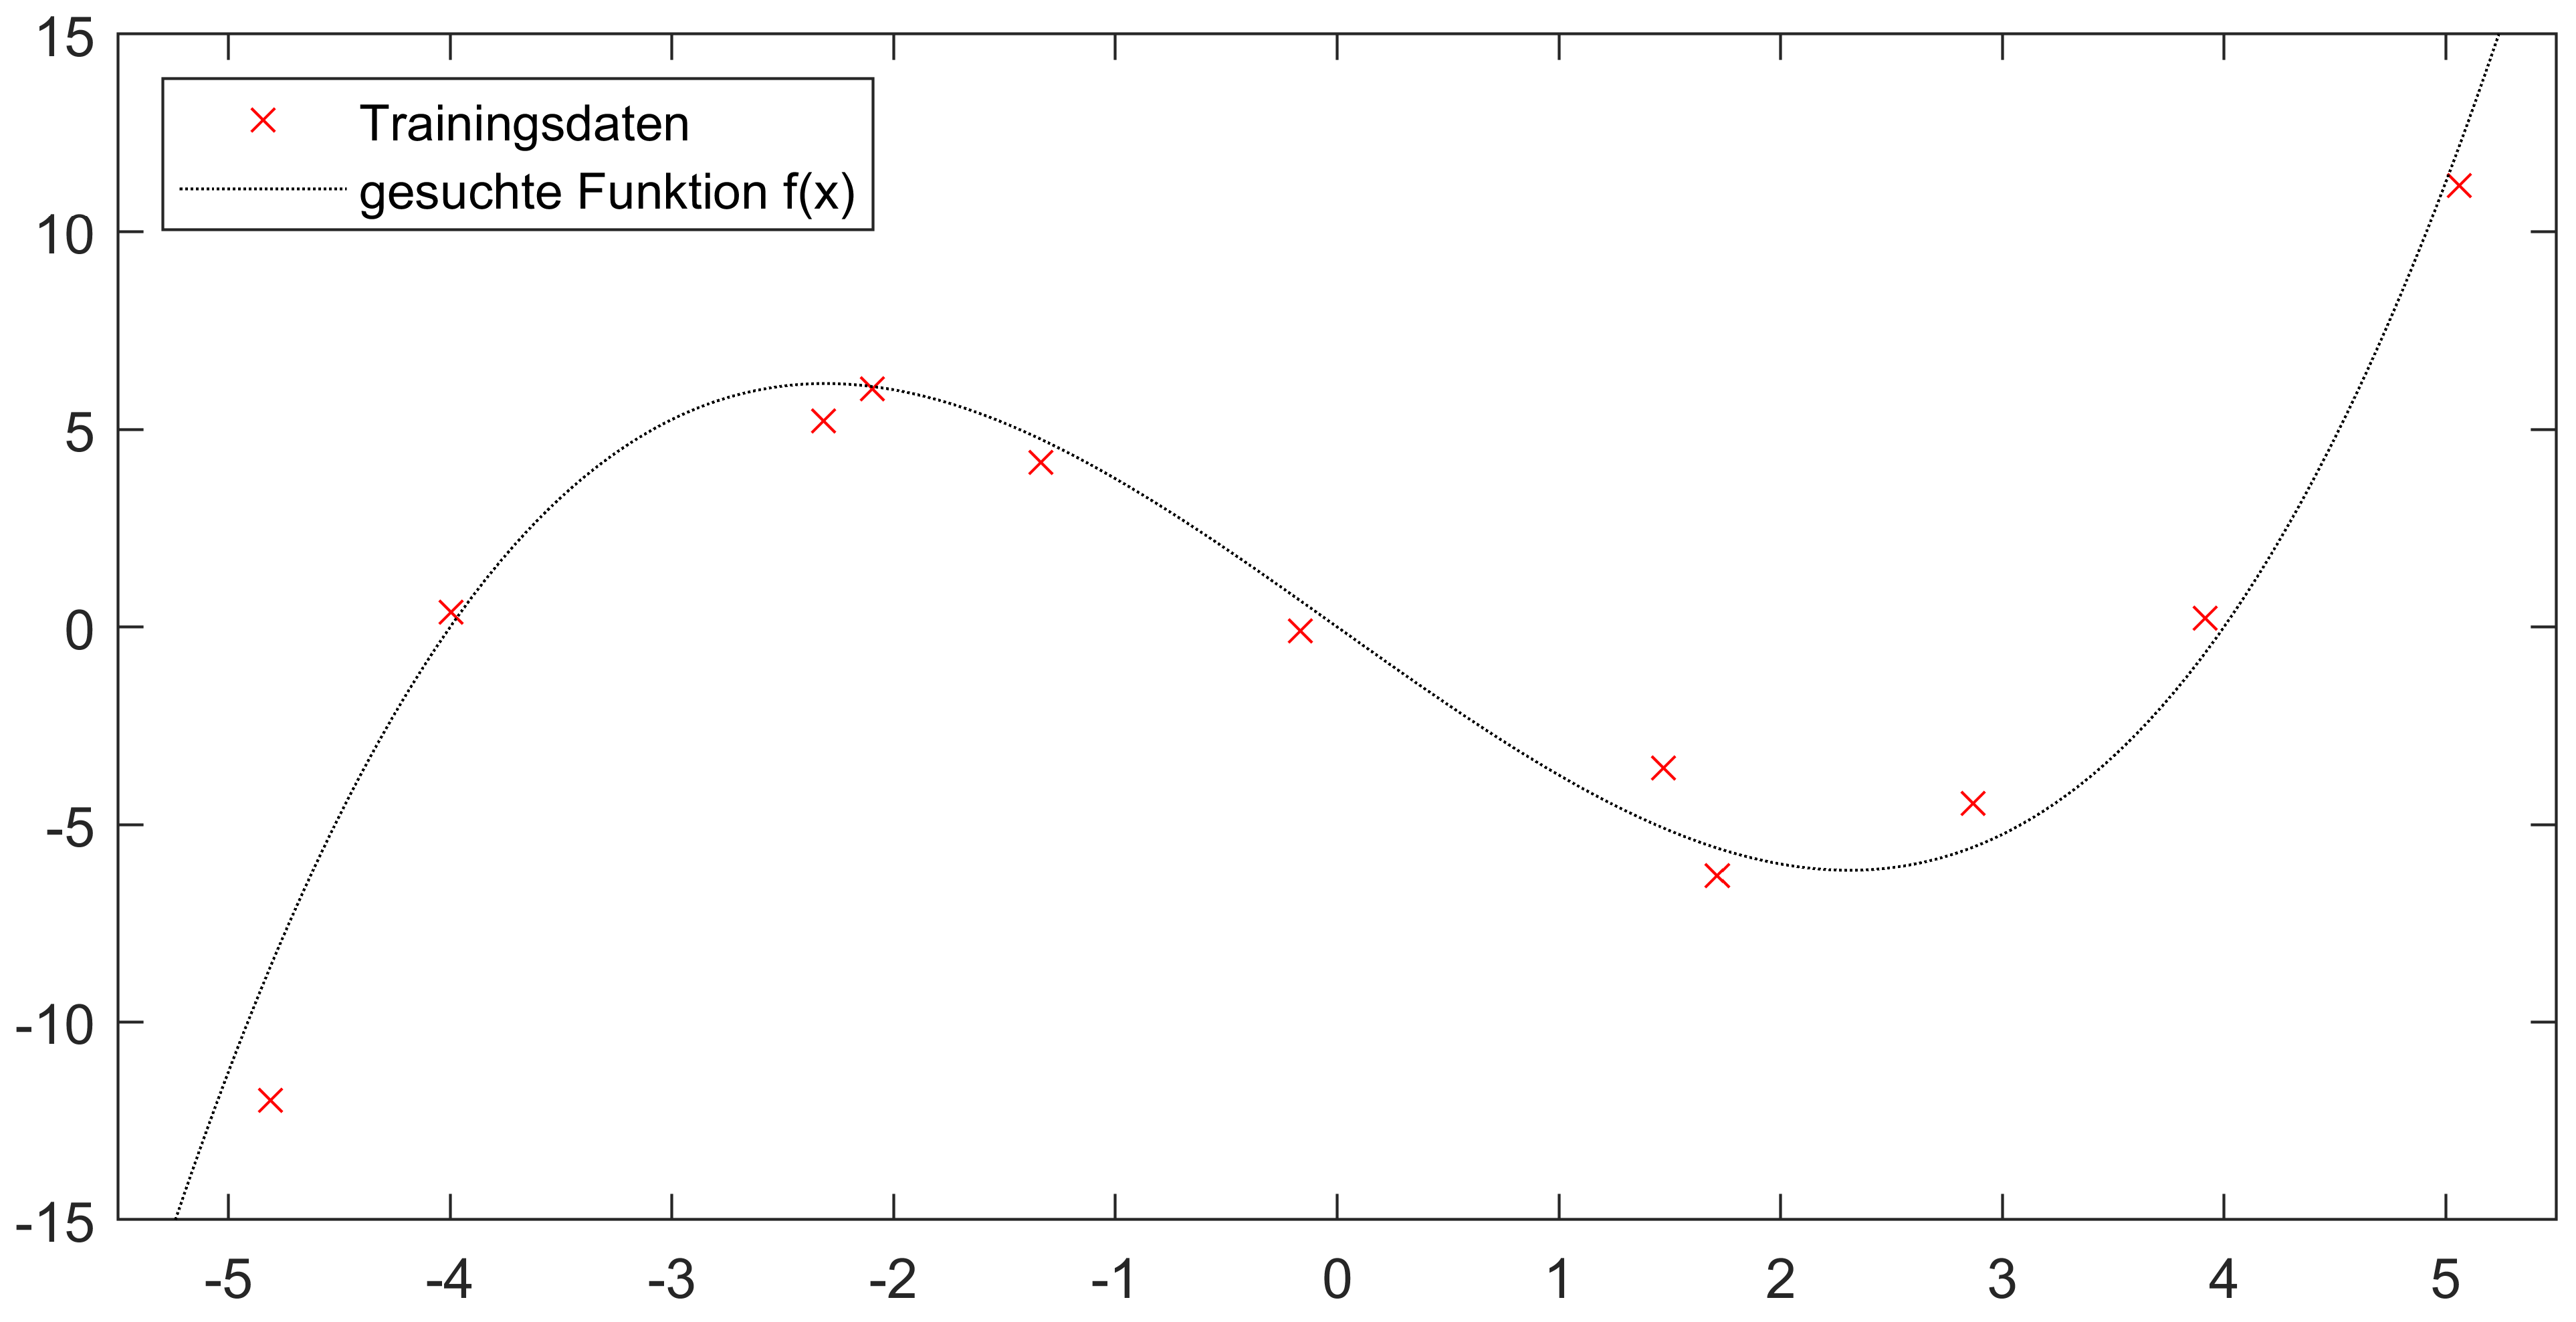
\includegraphics[width= 14cm]{fittingproblem}
	\caption[Beispiel zur Funktionsfindung]{Beispiel zur Funktionsfindung}
\end{figure}

$x$ und $y$ sollen dabei Werte von gesammelten Daten repräsentieren, weswegen mit einem natürlichen Rauschen der Daten zu rechnen ist. Nun gilt es mithilfe dieser Datenpunkte ein Modell zu finden, mit dem man einen $y$-Wert mit gegebenen $x$ bestimmen lässt. Zwar liesse sich dieses Problem auch mit \textit{KNN}s lösen, jedoch werden einfachheitshalber vorerst Polynomfunktionen zur Modellierung verwendet.

Bei 11 Datenpunkten kann ein Polynom zehnten Grades die Funktion folgendermassen modellieren:

\begin{figure}[h]
	\centering
	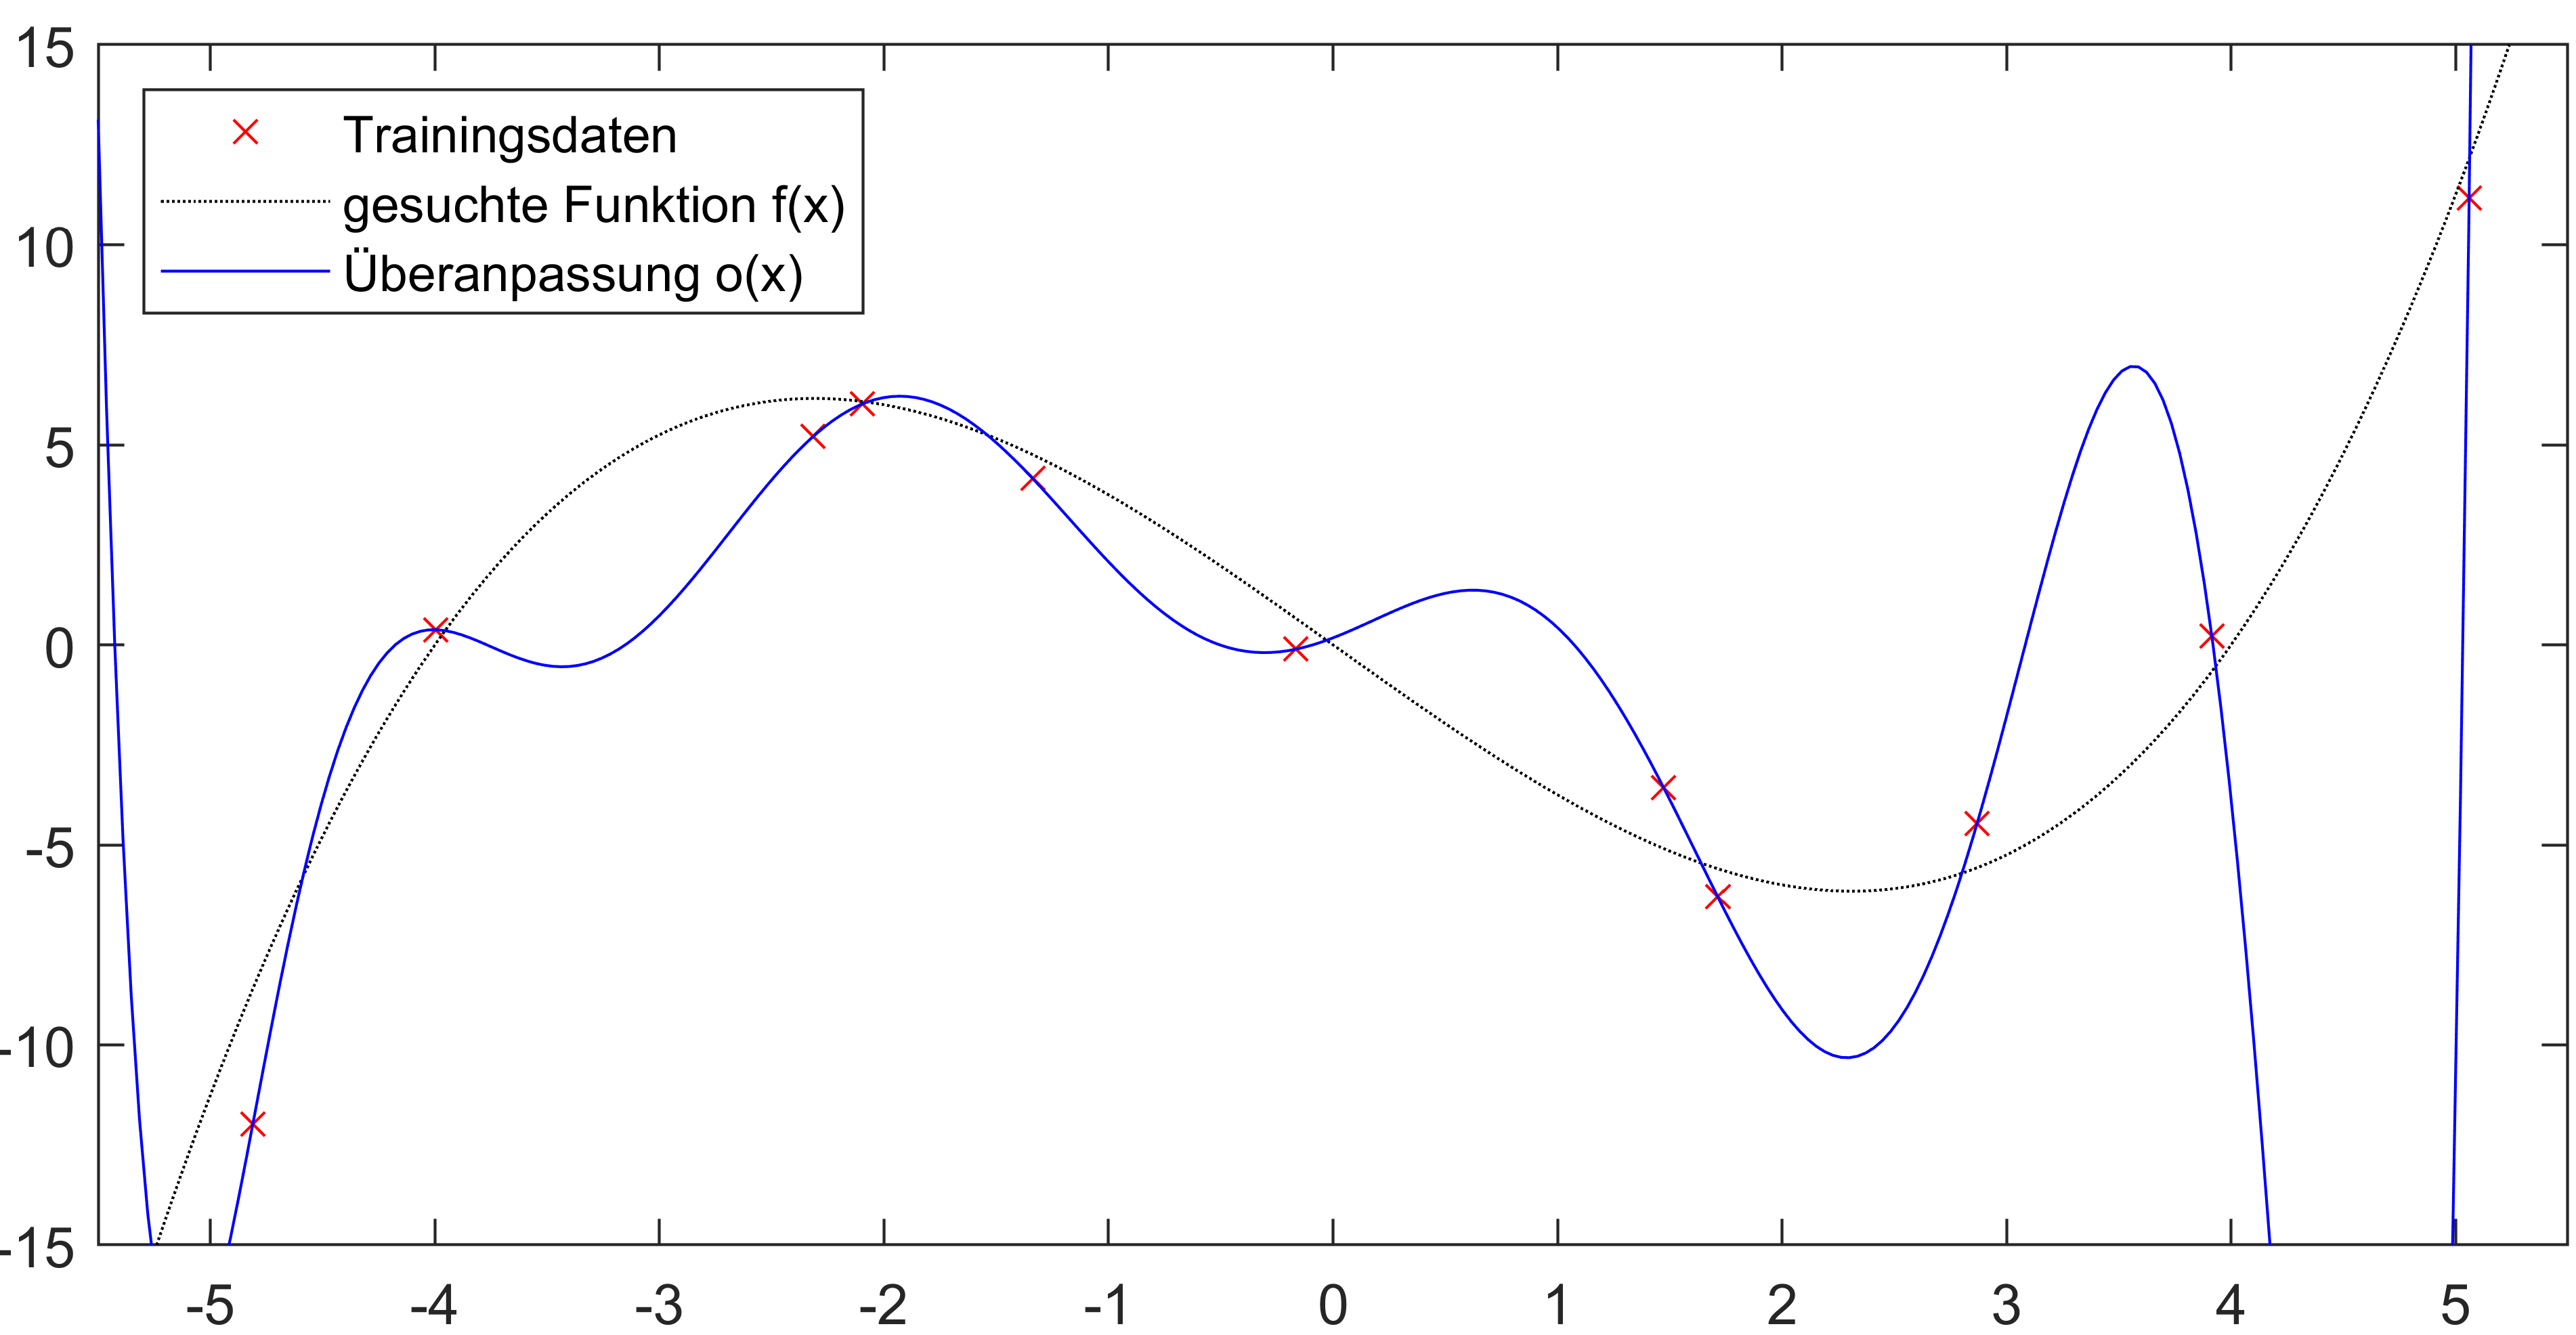
\includegraphics[width= 14cm]{overfitting}
	\caption[Beispiel mit Polynom 10. Grades]{Beispiel mit Polynom 10. Grades,  $\diameter$ Fehler Training: $0.00$}
\end{figure}

Die Funktionskurve $o(x)$ repräsentiert die gegebenen Datenpunkte zwar perfekt, jedoch stellt sich die Frage, ob  $o(x)$ auch ein Modell von der Unbekannten $f(x)$ ist. Wie gross ist die Wahrscheinlichkeit, dass $f(x) = o(x)$ und somit weitere Datenpunkte von $f(x)$ auch auf $o(x)$ zu liegen kommen? Wendet man $o(x)$ auf neue, ungelernte Daten an, erhält man folgenden Plot:

\begin{figure}[h]
	\centering
	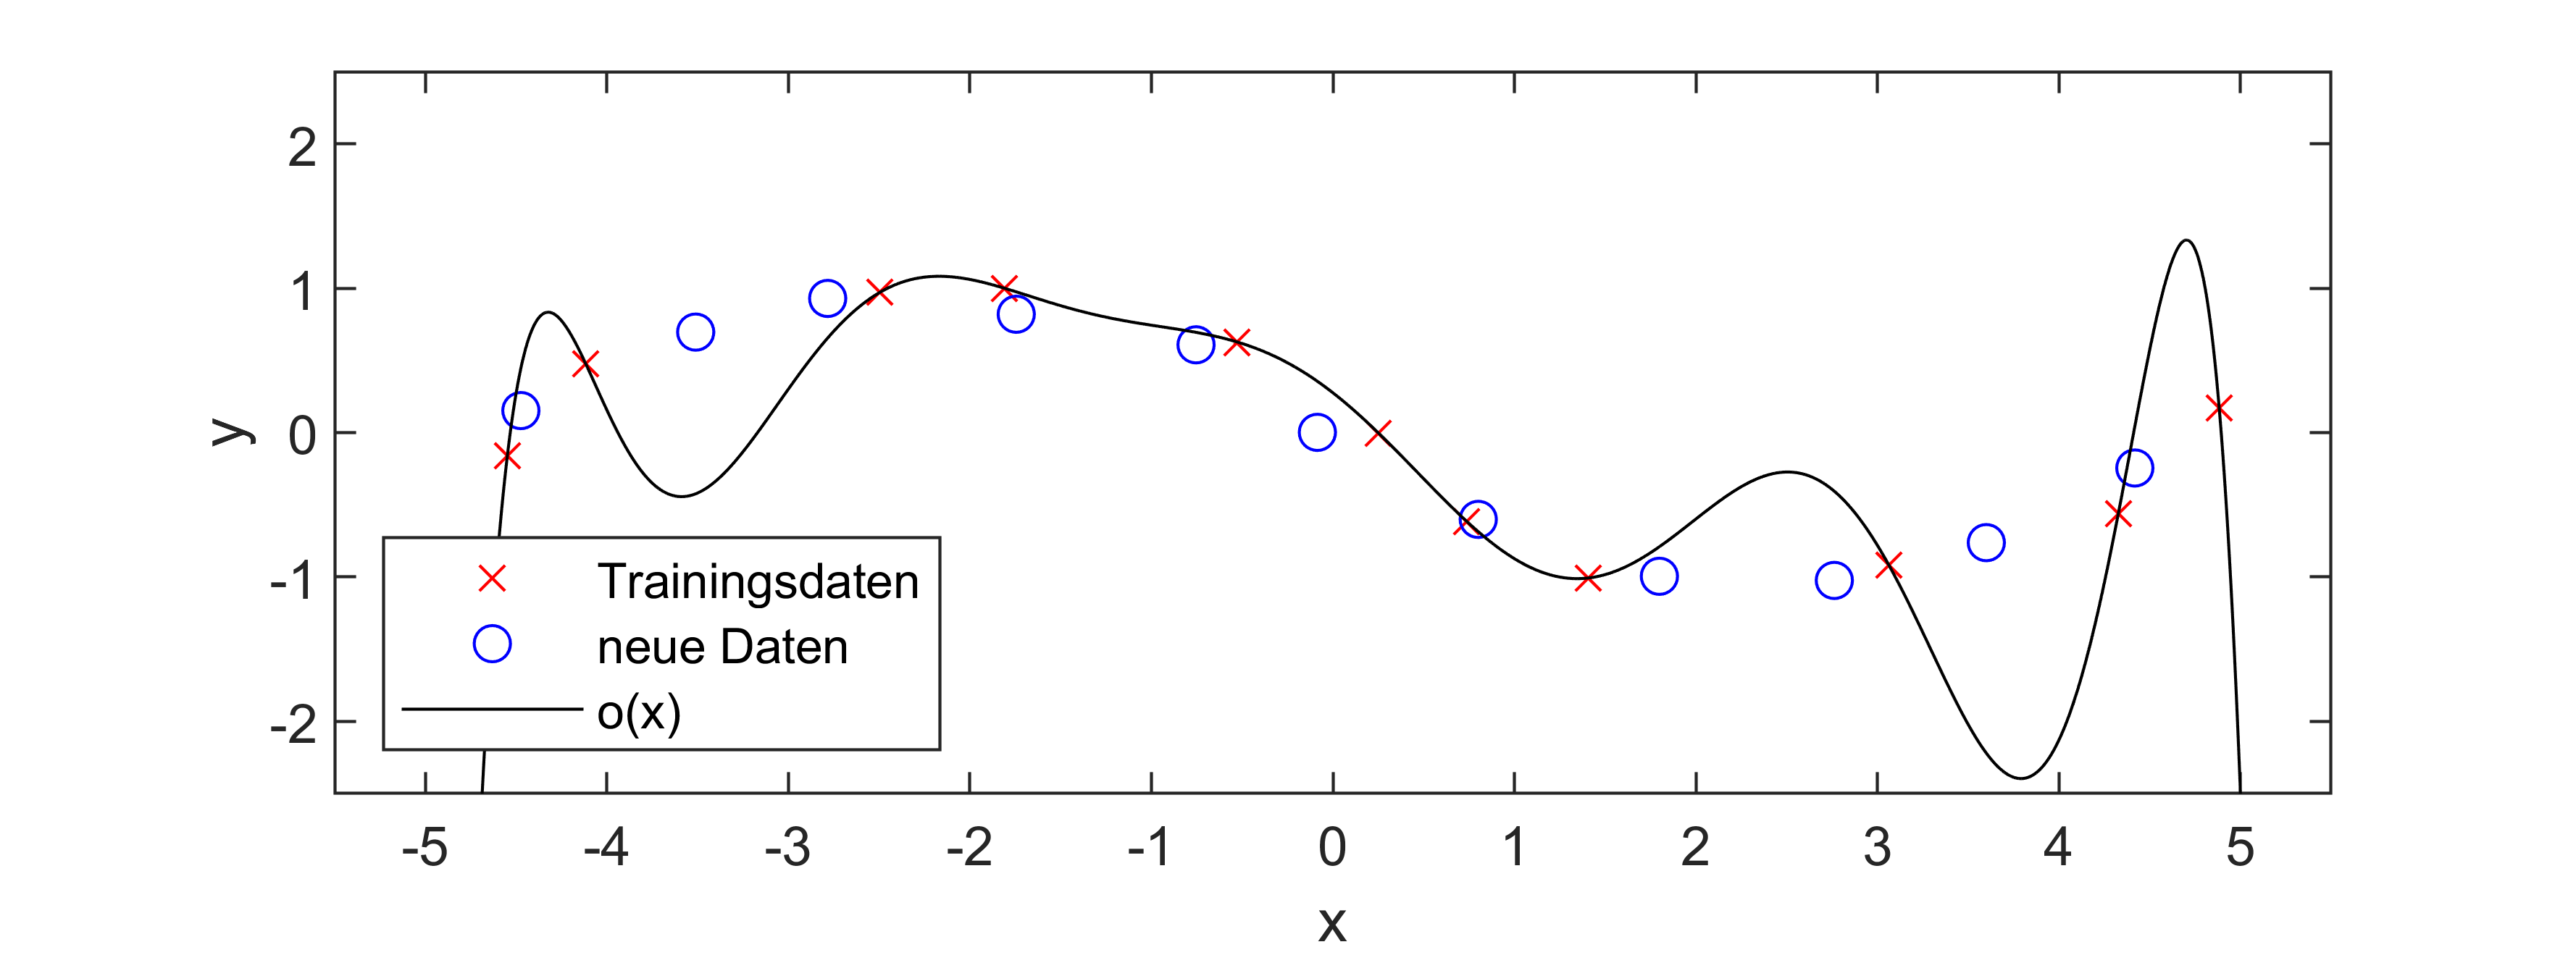
\includegraphics[width= 14cm]{overfitting_test}
	\caption[Beispiel mit Polynom 10. Grades mit neuen Datenpunkten]{Beispiel mit Polynom 10. Grades mit neuen Datenpunkten\\ $\diameter$ Fehler Training: $0.00$, $\diameter$ Fehler neu: $0.22$}
\end{figure}

Es stellt sich heraus, dass $f(x)$ keineswegs gleich $o(x)$ ist. Der Fehler der Trainingsdaten ist zwar klein, jedoch scheint $o(x)$ nicht auf neue Daten anwendbar zu sein.

\paragraph{Überanpassung} Erhält man ein verdächtig akkurates Ergebnis mit den Trainingsdaten, läuft man Gefahr der \textit{Überanpassung}: Der Algorithmus erstellt zu detaillierte Regeln für die Trainingsdaten spezifisch und verallgemeinert schlecht (er ''lernt auswendig''). \textit{Überanpassung} führt dazu, dass der Algorithmus zwar ausserordentliche Leistungen innerhalb der Trainingsdaten erzielt, jedoch ungelernte Daten nur mit einer sehr grossen Fehlerquote verarbeiten kann (siehe Beispiel in Abb. 4).

Um eine Überanpassung des Algorithmus zu vermeiden, verwendet man bei maschinellen Lernalgorithmen zwei sehr menschliche Eigenschaften:
\begin{itemize}[leftmargin=2cm]
	\item Gelegentlich Fehler machen dürfen
	\item Annahme, dass manche Eigenschaften ignoriert werden können
\end{itemize}
Wir selber würden diese wahrscheinlich als Schwäche bezeichnen, jedoch sind diese Eigenschaften Schlüssel für das \textit{maschinelle Lernen}. Sie erlauben es dem Algorithmus durch Weglassen von Details das Rauschen in den Trainingsdaten zu glätten. Es werden weniger Regeln aufgestellt, wodurch die Funktion weniger komplex wird. Die Reduktion der Komplexität führt aus rein probabilistischen Gründen dazu, dass der Algorithmus toleranter wird und somit verallgemeinert wird\cite{welch_prob}.

\begin{figure}[h]
	\centering
	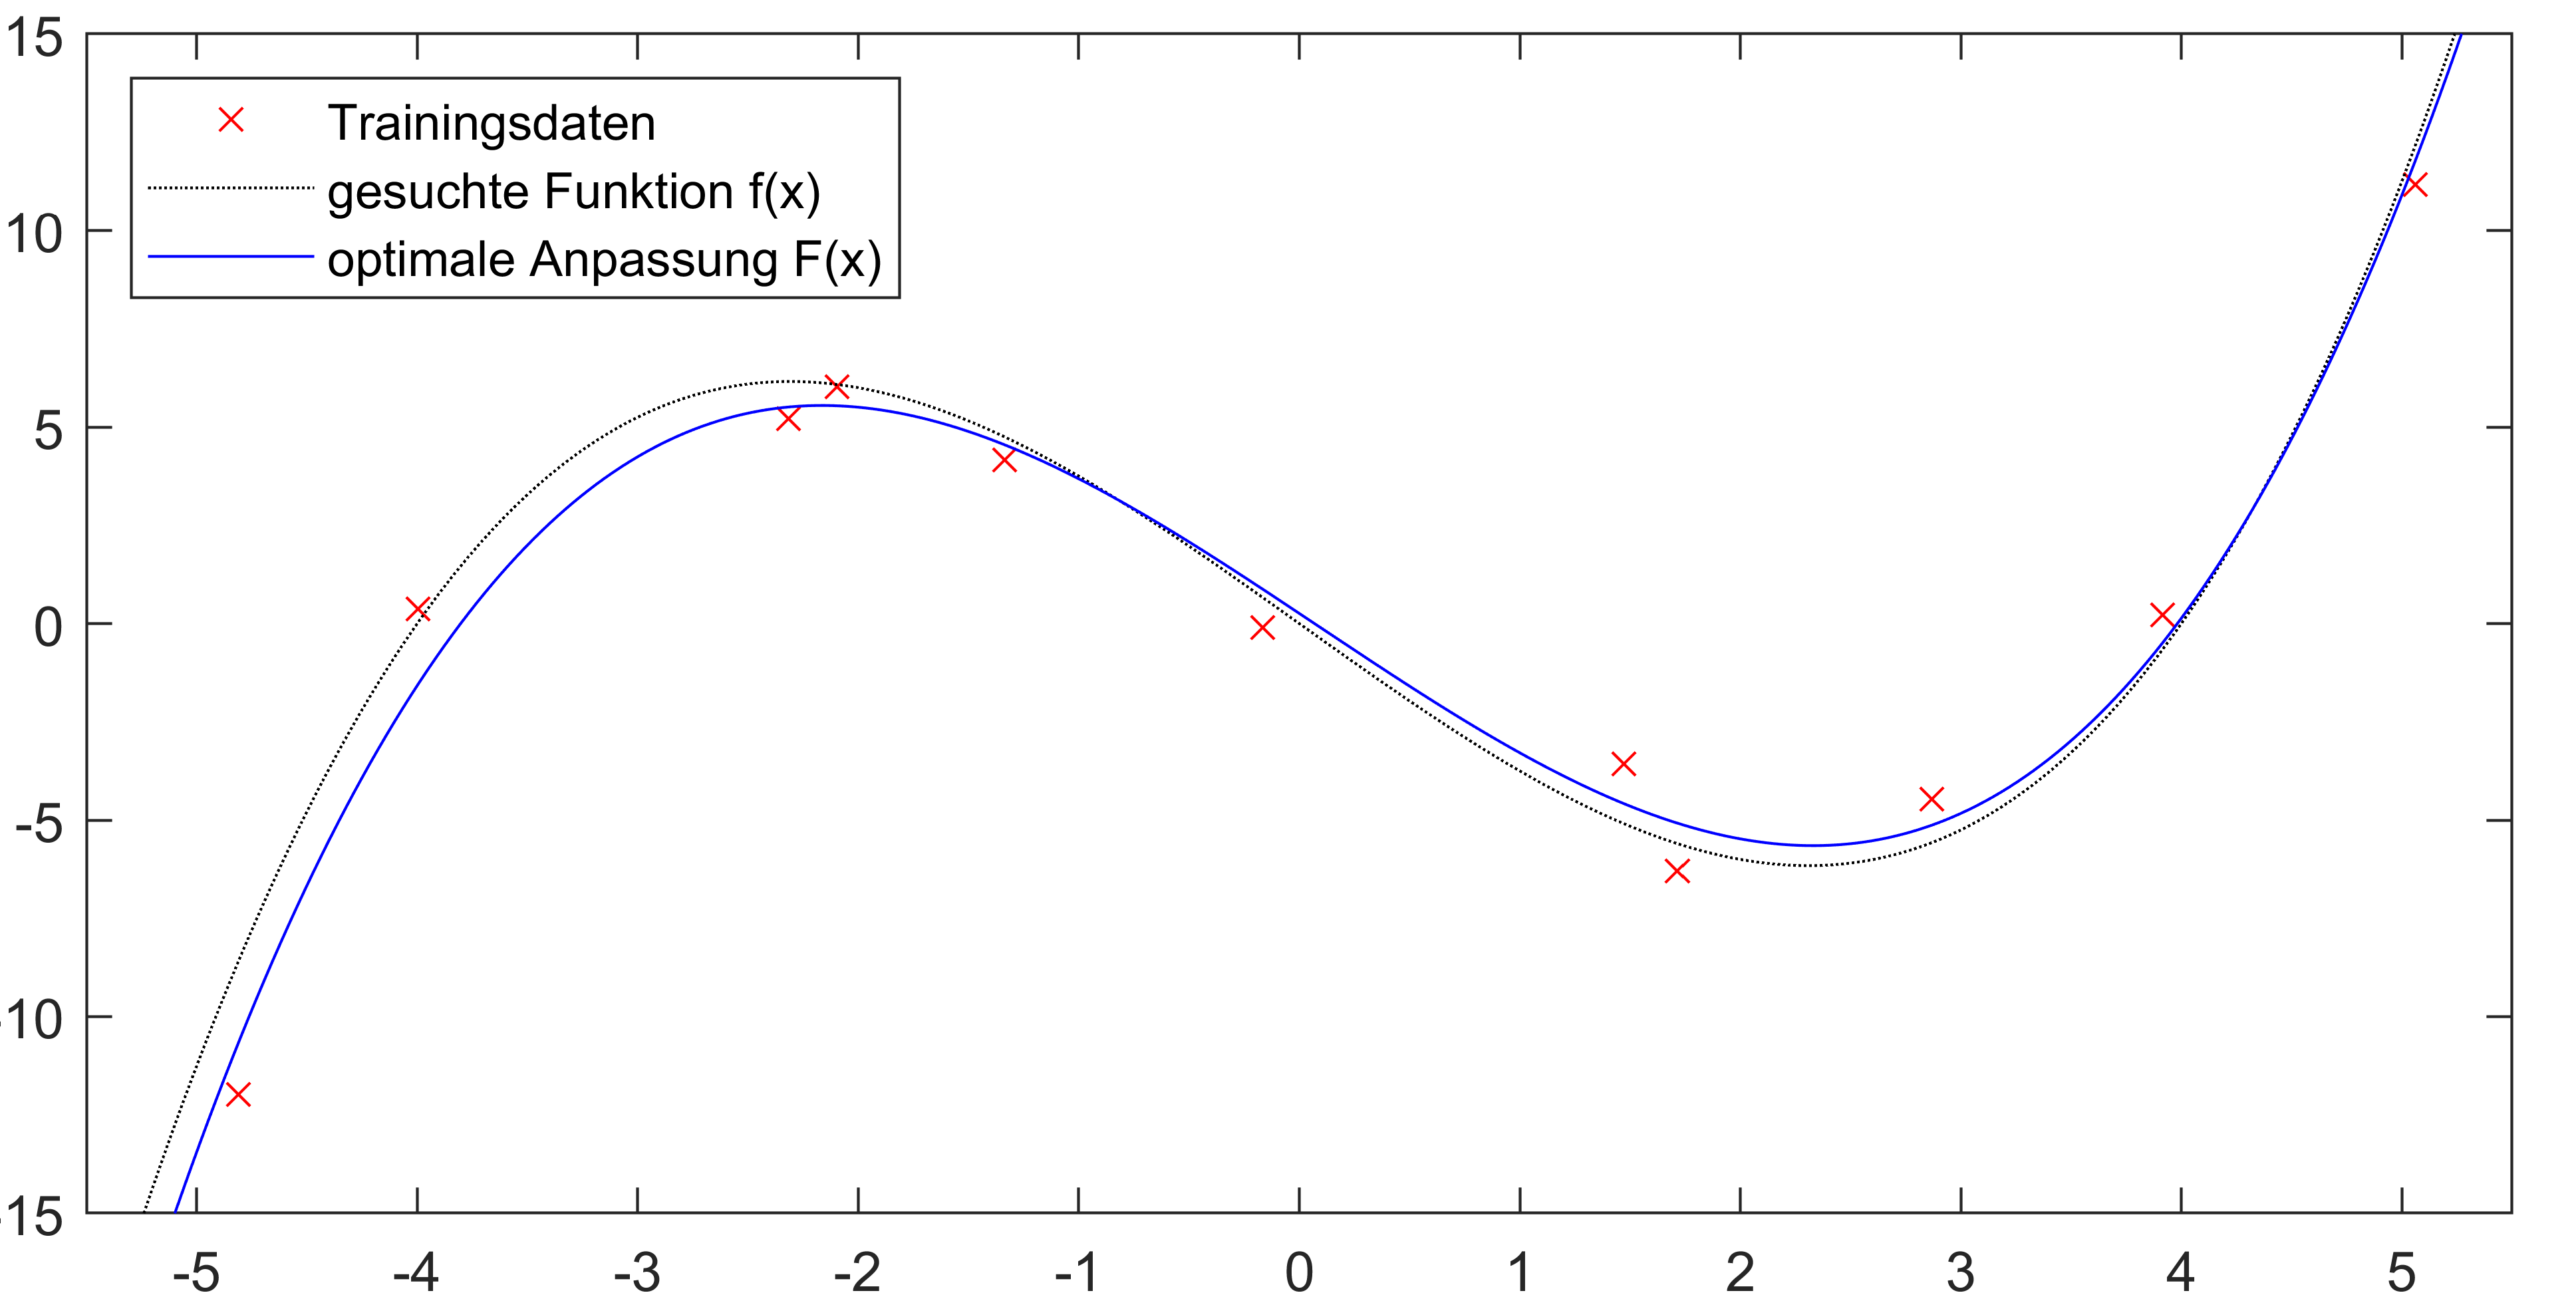
\includegraphics[width= 14cm]{fit}
	\caption[Beispiel mit Polynom 3. Grades]{Beispiel mit Polynom 3. Grades, $\diameter$ Fehler Training: $0.11$, $\diameter$ Fehler neu: $0.12$}
\end{figure}

Die ähnlichen Fehlerwerte von Trainingsdaten sowie den neuen Daten weist darauf hin, dass ein Polynom 3. Grades die Unbekannte $f(s)$ besser repräsentiert als $o(x)$. Mit $F(x)$ können somit auch neue Datenpunkte zuverlässig bestimmt werden.

\paragraph{Unteranpassung} Wenn man nun aber zu viele Annahmen und Fehler zulässt, unterliegt man der Gefahr der \textit{Unteranpassung}, bei der die Leistung des Algorithmus über alle gelernten sowie ungelernten Daten konsistent schlecht ist: Der Algorithmus verallgemeinert zwar sehr gut, aber macht zu viele/falsche Annahmen und ignoriert für die Bestimmung relevante Details. Unteranpassung tritt dann auf, wenn der Algorithmus zu simpel ist oder unpassend für die Problemstellung designet worden ist.\\

\begin{figure}[h]
	\centering
	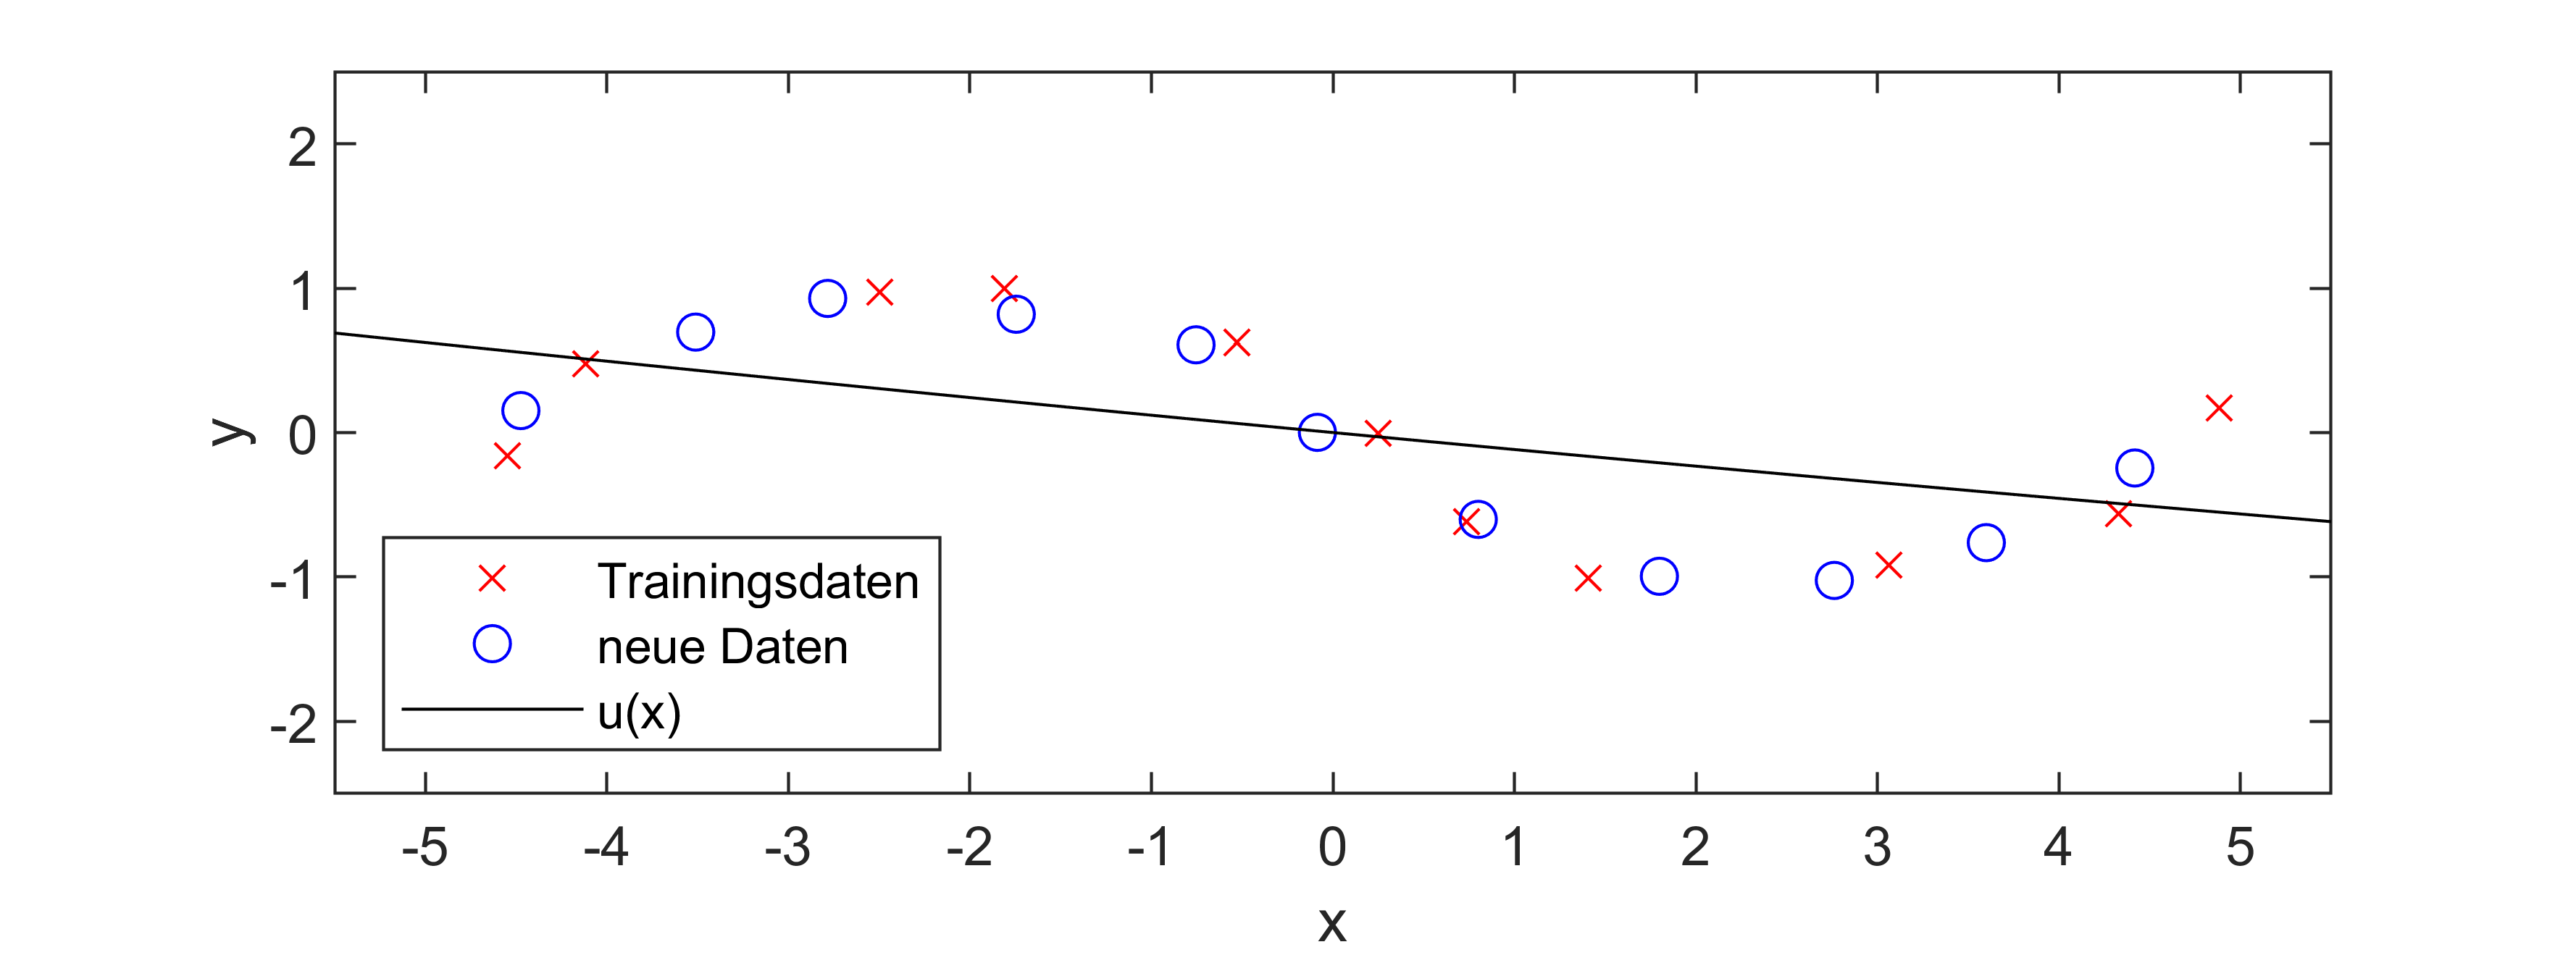
\includegraphics[width= 14cm]{underfitting}
	\caption[Beispiel mit Polynom 2. Grades]{Beispiel mit Polynom 2. Grades $\diameter$ Fehler Training: $0.50$, $\diameter$ Fehler neu: $0.45$}
\end{figure}

Für das Beispiel bedeutet eine Unteranpassung, dass die Funktion $u(x)$ zu einfach ist (Polynom 2. Grades), um weder die Trainingsdaten noch neue Daten akkurat modellieren zu können.

\paragraph{Validierung} Will man einen Lernalgorithmus allgemein anwendbar trainieren, ist auf die richtige Balance zwischen Einfachheit (\textit{Verzerrung}) und Komplexität (\textit{Varianz}) zu achten, wobei \textit{Überanpassung} als auch \textit{Unteranpassung} vermieden werden sollten. Um dies zu gewährleisten, werden während dem Training regelmässig Validierungsdaten eingespeist, auf welche der Algorithmus \textbf{nicht} trainiert wird. Mit den durch die Validierungsdaten gelieferten Ergebnissen kann auf die Leistung des Algorithmus ausserhalb der Trainingsumgebung geschlossen werden. Sobald die Leistung mit den Validierungsdaten sinkt während die der Trainingsdaten weiterhin steigt, kann man davon ausgehen, dass der Algorithmus ein Optimum erreicht hat und dass weiteres Trainieren zu einer Überanpassung führen wird. Wenn der trainierte Algorithmus in seinem Optimum trotzdem keine zufriedenstellenden Ergebnisse liefert, ist von einer \textit{Unteranpassung} auszugehen. Durch Ändern der Trainingsparameter\footnotemark oder durch Umgestaltung des Algorithmus kann der \textit{Unteranpassung} aber auch der \textit{Überanpassung} entgegengewirkt werden.

\footnotetext{\label{fn:meta}Nicht zu verwechseln mit den \textit{Parametern} des Algorithmus! Trainingsparameter beeinflussen den Trainingsprozess, d.h. Dauer des Trainings, Anzahl Trainings-/Validierungsdaten, etc. Die \textit{Parameter} des Algorithmus werden trainiert und berechnen aus den Eingangsdaten Ausgangsdaten. Um die Verwechslung dieser beiden relevanten Begriffe zu vermeiden, wird für die Trainingsparameter wie auch für die Architektur des Algorithmus der Begriff \textbf{Meta-Parameter} verwendet.}

\subsection[KNNs]{Künstliche neuronale Netze}
Obwohl die \textit{KNN}s erst in den letzten Jahren ihren grossen Durchbruch erlebt hatten, lässt sich die ursprüngliche Idee von \textit{künstlichen neuronalen Netzen} bis in die 40er Jahre zurückdatieren. In den 50er Jahren wurden die ersten Versuche mit Rechnern der damaligen Zeit durchgeführt, wobei mit dem Vorgänger des \textit{Neurons}, dem \textit{Perceptron}, nur müssiger Fortschritt erzielt worden ist. Erst mit der Entwicklung der sehr effizienten \textit{Gradient Descent-Trainingsmethode} und der Einführung der heute gängigen \textit{Neuronen} kam die Forschung an \textit{KNN}s in den 70er Jahren wieder in Fahrt. Der richtige Durchbruch der \textit{KNN}s kam aber erst in den letzten beiden Jahrzehnten mit der rapiden Steigerung der Prozessorleistung, aber auch dem Aufkommen des Internets und der schieren Menge an gespeicherten und zugänglichen Daten. Das ermöglichte mit neuen Entwicklungen im Bereich des \textit{Deep Learnings} höchst komplexe Systeme. So waren solche \textit{DNN}s in der Lage, Aufgaben zu meistern, welche für Algorithmen lange als sehr schwierig oder unmöglich erachtet worden sind. Mit neusten Erfolgen in der Bilderkennung, aber auch der Entscheidungsfindung (siehe Kapitel 1 \textit{AlphaGo}) und vielen praktischen Anwendungen hat \textit{Deep Learning} öffentliche Aufmerksamkeit erhalten\cite{ann}.\\

Die technischen Informationen zu \textit{KNN}s und \textit{DNN}s in den folgenden Abschnitten sowie im Kapitel \ref{cha:theo:dl} basieren auf dem öffentlich verfügbaren Lernmittel \textit{Neural Networks and Deep Learning} von Michael Nielsen\cite{nielsen}.

\subsubsection{Die Natur als Vorbild}
Um die in Kapitel \ref{cha:theo:ml} erwähnten Lernverhalten simulieren zu können, bedienen sich die \textit{KNN}s dem Vorbild der Natur: das Gehirn. Die Lernfähigkeit des Gehirns lässt sich in wenigen Worten folgendermassen formulieren: Das menschliche Gehirn besteht aus etwa 15 Milliarden Neuronen, welche durch  Verbindungen miteinander vernetzt sind. Diese Neuronen sind in der Lage, Signale aus den eingehenden Verbindungen mittels Ionenkanäle zu gewichten und mithilfe der in der Zelle herrschenden Ladung miteinander zu verrechnen. Sobald die Ladung einen gewissen Schwellenwert übersteigt, feuert das Neuron und gibt das Signal an die folgenden Neuronen weiter, welche den selben Prozess wiederholen. Der Lernprozess wird durch Belohnung von nützlichen und häufig verwendeten Verbindungen bewerkstelligt, wobei diese Verbindungen verstärkt und stärker gewichtet werden und ungebrauchte oder ungünstige Verbindungen verkümmern\cite{klett}.

Auf diesen Grundlagen basiert die Idee der \textit{KNN}s, weswegen sie auch noch eine weitere wichtige Eingenschaft gemeinsam haben: Als Aussenstehender ist einem genaue das genaue Funktionsprinzip unbekannt. So sind wir wie auch \textit{KNN}s dazu fähig, handschriftliche Ziffern voneinander zu unterscheiden, wie es aber im Detail bewerkstelligt wird, ist und bleibt unklar\footnote{Ironischerweise war eine Motivation für die Entwicklung von \textit{KNN}s, uns ein besseres Verständnis für die Funktionsweise von intelligentem Verhalten zu geben. Jedoch stellte es sich heraus, dass weder \textit{KNN}s noch das biologische Vorbild im Detail verstanden werden können.}. Für die algorithmische Umsetzung wurden jedoch einige Anpassungen vorgenommen, daher sind heutige \textit{KNN}s nur noch im entferntesten Sinne mit biologischen neuronalen Netzen verwandt. 

\subsubsection{Neuronen \& Verbindungen}\label{cha:theo:neurons}
Das \textit{Neuron} ist der Grundbaustein von \textit{KNN}s. Wie das biologische Vorbild enthält es mehrere Signaleingänge sowie einen Signalausgang, alle Eingangssignale werden mit einem Faktor Gewichtet und zudem hat jedes \textit{Neuron} seinen Schwellenwert. Die Gewichtungen wie auch der Schwellenwert sind die zu trainierenden \textit{Parameter} des \textit{KNN}s.
\begin{figure}[h]
	\centering
	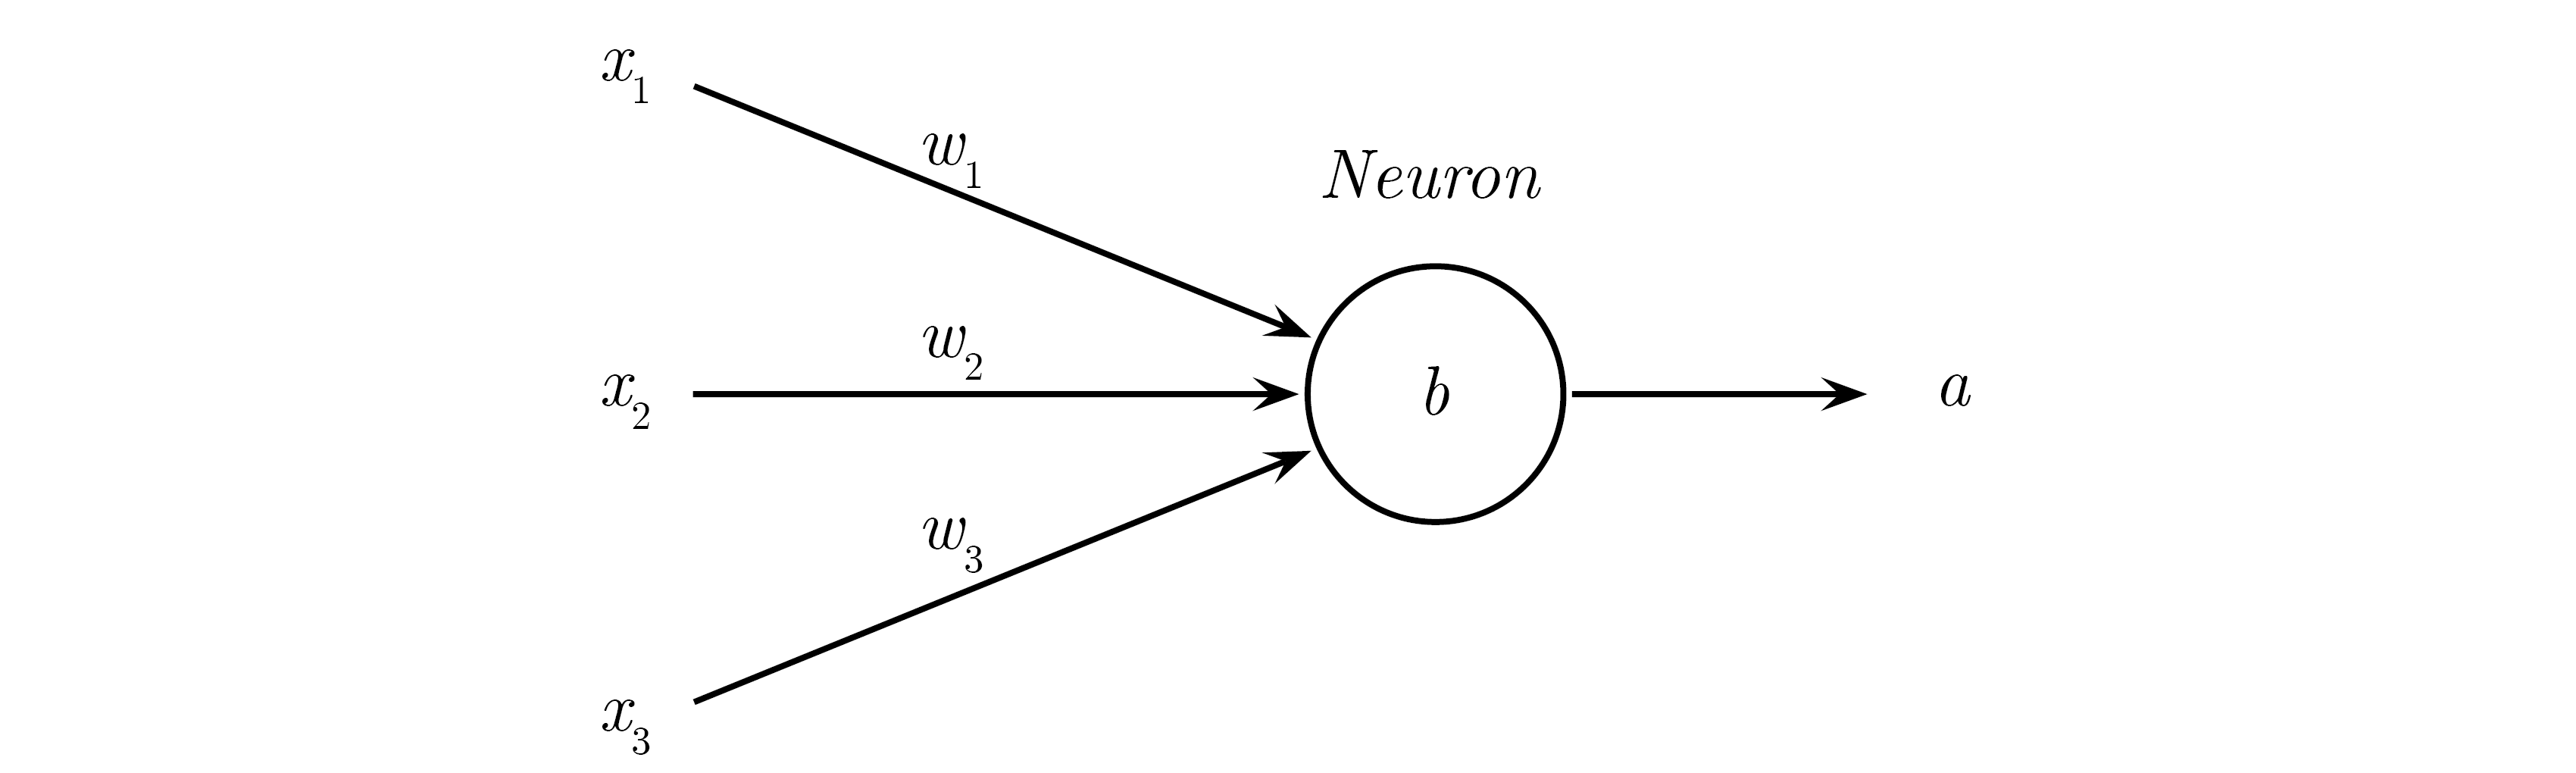
\includegraphics[width=\textwidth]{single_neuron}
	\caption[Schema von einem künstlichen Neuron]{Schema von einem künstlichen Neuron}
	\label{img:single_neuron}
\end{figure}

Den Eingangssignalen werden die Variablen  $x_1, x_2,...,x_n$ gegeben, wobei sie jeden Wert zwischen $1$ und $0$ annehmen können. Zur Verallgemeinerung der Formeln wird $n$ für die Anzahl der Eingangssignale verwendet. Jeder Verbindung wird ein Gewichtungs-\textit{Parameter} $w_1, w_2,...,w_n$\footnotemark gegeben, dessen Zahlenwert nicht begrenzt ist und daher auch negativ sein kann. Die Eingangssignale werden mit dem jeweiligen Gewichtungs-\textit{Parameter} multipliziert ($x_i\cdot w_i$), wodurch man das gewichtete Signal vom $i$-ten Eingang erhält. Im nächsten Schritt gilt es, alle gewichteten Signale zu summieren, welches in folgender Formel bewerkstelligt wird:

\footnotetext{In den folgenden Kapiteln werden die Gewichtungen $w_1, w_2,...,w_n$ und der Schwellenwert $b$ eines Neurons allgemein als \textbf{Parameter} bezeichnet. Nicht zu verwechseln mit den \textbf{Meta-Parametern}(siehe Fussnote \ref{fn:meta})}
	
\begin{equation}\label{eq:weighted_input}
	\sum_{i=1}^{n} x_i\cdot w_i
\end{equation}
Nun soll der Schwellenwert-\textit{Parameter} $b$\footnotemark[\value{footnote}]  implementiert werden. $b$ wird mit dem Ergebnis der Formel \ref{eq:weighted_input} verglichen, womit der Ausgang $a$ steuern soll. Da der Ausgang $a$ für die Aufbau eines \textit{KNN}s wiederum als Eingangssignal von einem anderen \textit{Neuron} verwendet wird, soll wieder $0\leq a \leq 1$ gelten. Der Begriff ''Schwellenwert'' würde auf dieses Problem folgende Beziehung implizieren:
\begin{center}
	\begin{minipage}{7cm}
		wenn $\sum_{i}x_iw_i < b$ dann $a=1$\\
		wenn $\sum_{i}x_iw_i > b$ dann $a=0$
	\end{minipage}
\end{center}
was dem selben Entspricht wie
\begin{center}
\begin{minipage}{7cm}
	wenn $\sum_{i}x_iw_i - b < 0$ dann $a=1$\\
	wenn $\sum_{i}x_iw_i - b > 0$ dann $a=0$
\end{minipage}
\end{center}
Mit dieser Annahme trifft man sogleich auf zwei Ungereimtheiten in den Konventionen der \textit{KNN}s. Die erste ist rein Formal: $b$ soll definiert werden als $b \equiv$ -Schwellenwert, wodurch das Vorzeichen von $b$ gewechselt werden kann:
\begin{center}
	\begin{minipage}{7cm}
		wenn $\sum_{i}x_iw_i + b < 0$ dann $a=1$\\
		wenn $\sum_{i}x_iw_i + b > 0$ dann $a=0$
	\end{minipage}
\end{center}
An dieser Stelle soll zur Übersicht der linke Term der Ungleichung $\sum_{i=1}^{n} x_i\cdot w_i+b$ gleich zur Variable $z$ zusammengefasst werden:
\begin{equation}\label{eq:def_z}
\sum_{i=1}^{n} x_i\cdot w_i+b\equiv z
\end{equation}
Die Zweite Änderung betrifft den digitalen Wechsel zwischen den $0$ und $1$ vom Ausgangswert $a$, sobald der Schwellenwert überschritten wird. Für das Ergebnis $a$ des Neurons sähe der Funktionsgraph in Relation zur neuen Variable $z$, welche für die gewichtete Summe abzüglich des Schwellenwertes steht, folgendermassen aus:

\begin{figure}[h]
	\centering
	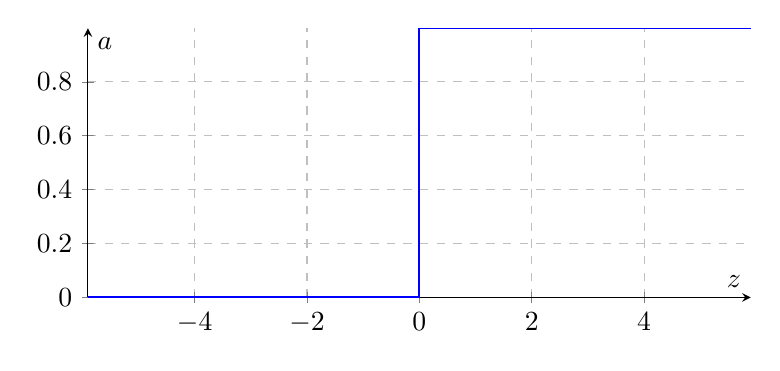
\begin{tikzpicture}
	\begin{axis}[
	xlabel={$z$},
	ylabel={$a$},
	xmin=-5.9, xmax=5.9,
	ymin=0, ymax=0.999,
	ymajorgrids=true,
	xmajorgrids=true,
	grid style=dashed,
	width=10cm,
	height=5cm,
	axis line style = <->,
	axis lines=middle,
	axis x line=bottom,
	axis y line=left
	]
	\addplot+[const plot, no marks, thick] coordinates {(-6,0) (0,0.999) (6,0.999)};
	\end{axis}
	\end{tikzpicture}
	\caption[Stufen-Funktion]{Stufen-Funktion step$(z) = a$}
	\label{plt:step}
\end{figure}
Da die Stufen-Funktion nicht differenzierbar ist und nirgends einen Gradienten aufweist, kann sie nicht in einem \textit{KNN} eingesetzt werden. Statt den Schwellenwert $-b$ also als klare Grenze zu nehmen, muss ein stufenloser Wechsel zwischen $0$ und $1$ ermöglicht werden. Die \textit{Sigmoid}-Funktion\footnote{Definition der \textit{Sigmoid}-Funktion: $\sigma(x) = \frac{1}{1+e^{-x}}$} $\sigma(z)$ ist die gängigste Funktion, die diese Eigenschaften erfüllt: 


\begin{figure}[h]
	\centering
	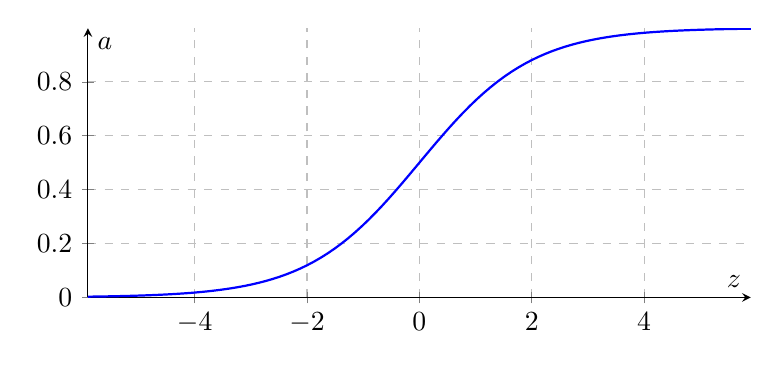
\begin{tikzpicture}
	\begin{axis}[
	xlabel={$z$},
	ylabel={$a$},
	xmin=-5.9, xmax=5.9,
	ymin=0, ymax=0.999,
	ymajorgrids=true,
	xmajorgrids=true,
	grid style=dashed,
	width=10cm,
	height=5cm,
	axis line style = <->,
	axis lines=middle,
	axis x line=bottom,
	axis y line=left
	]
	\addplot[-, thick, blue] expression[domain=-6:6,samples=100]{(1+(2.7182818^(-x)))^(-1)}; 
	
	\end{axis}
	\end{tikzpicture}
	\caption[Sigmoid-Funktion]{Sigmoid-Funktion $\sigma(z) = a$}
	\label{plt:sigmoid}
\end{figure}
Mit der \textit{Sigmoid}-Funktion als ideale Kurve zur Standardisierung von $z$ gilt es nur noch, alle Elemente miteinander zu verknüpfen:


\begin{equation}\label{eq:neuron_eq}
a = \sigma \left( \sum_{i=1}^{n} x_i\cdot w_i+b\right)  \qquad \text{oder} \qquad a = \sigma \left( z \right)
\vspace*{2mm}
\end{equation}

Dies ist die Formel eines jeden \textit{Neurons} und bildet (z.T. mit geringfügigen Modifikationen) den Grundbaustein aller \textit{KNN}s.\\

Anzumerken ist, dass die Formel \ref{eq:neuron_eq} eine ganz normale Funktion ist, welche den Eingangswerten $x_1,...,x_n$ einen Ausgangswert $a$ zuordnet. Die Variablen $w_1,...,w_n$ und $b$ sind \textit{Parameter} und werden nicht von den Eingangsdaten beeinflusst.

Auch ist hinzuzufügen, dass die Funktion \ref{eq:neuron_eq} aufgrund der \textit{Glätte} der \textit{Sigmoid}-Kurve und der Linearität der restlichen Operationen ebenfalls differenzierbar ist. Diese Eingenschaft wird später essenziell, um einen effizienten Trainingsalgorithmus für die Justierung der \textit{Parameter} zu entwickeln.

\subsubsection{Layers}\label{cha:theo:layers}

Da ein einzelnes \textit{Neuron} alleine nicht viel leisten kann, werden sie miteinander vernetzt --- daher auch der Name \textit{künstliches neuronales Netz}. Die gängigste Art schlägt folgende Vernetzung vor:

\begin{figure}[h]
	\centering
	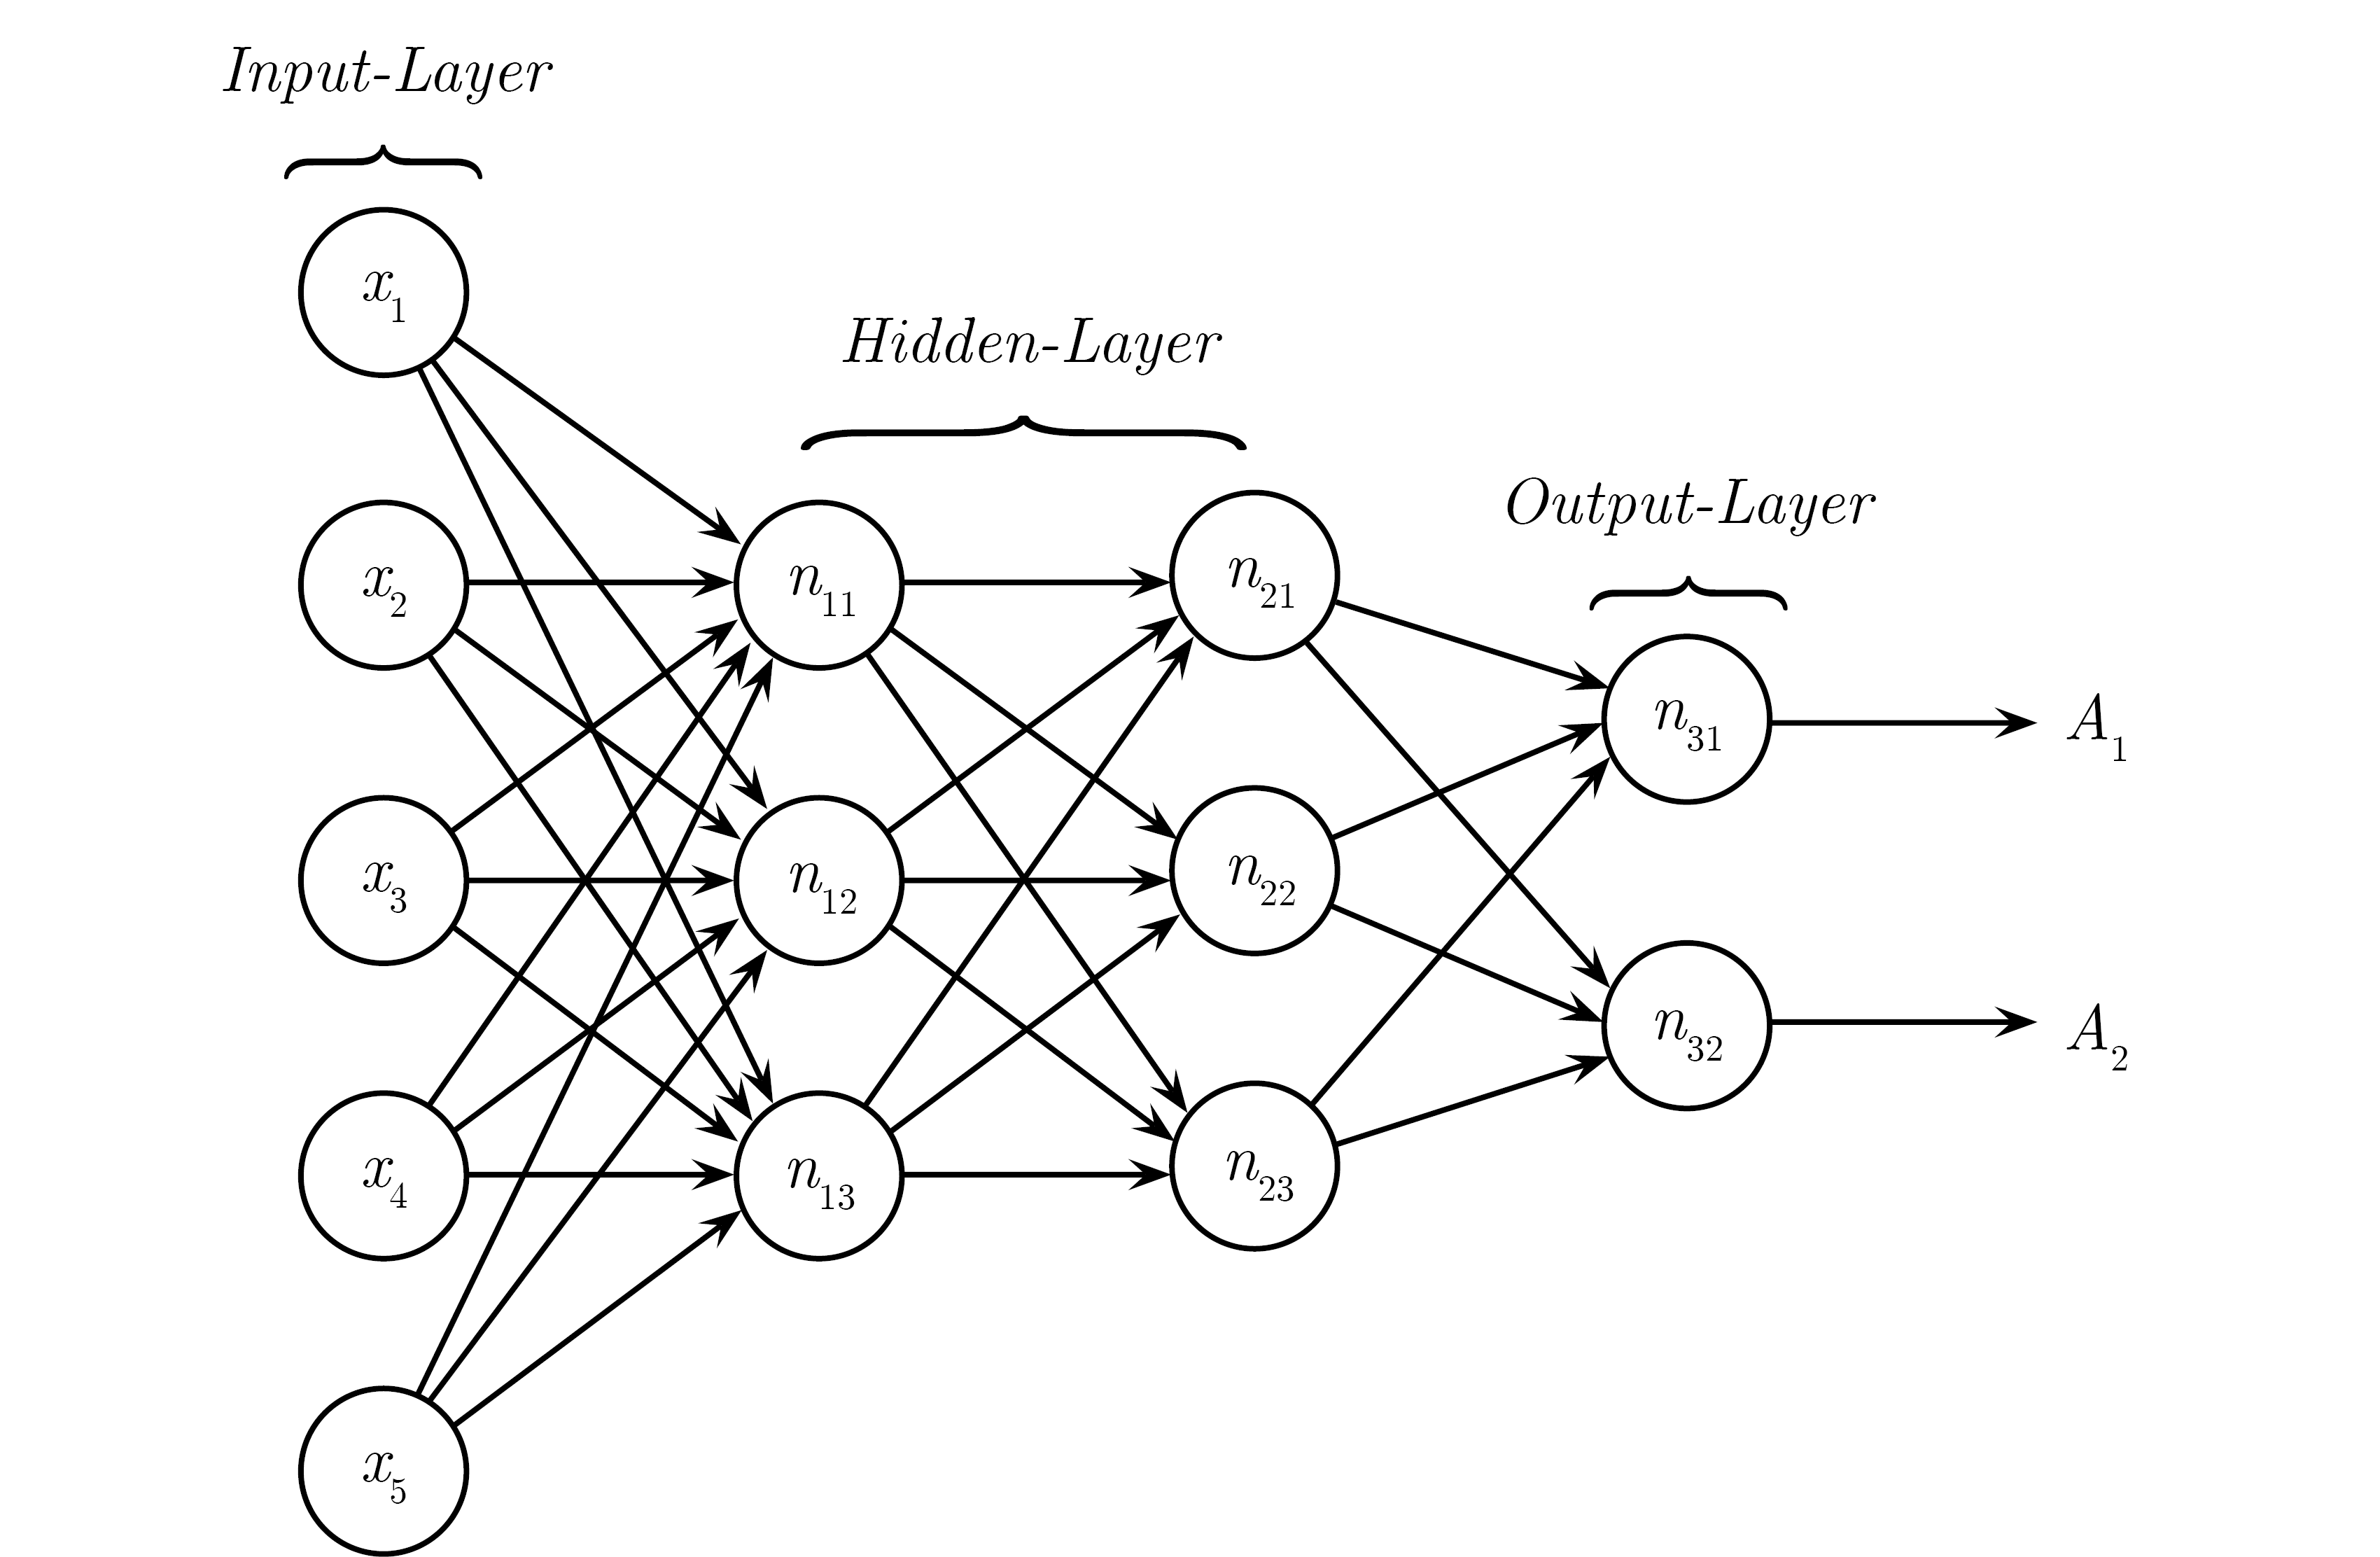
\includegraphics[width=\textwidth]{layers}
	\caption[Schema von kleinem \textit{KNN}]{Schema von einem kleinen \textit{KNN}}
	\label{img:layers}
\end{figure}

Die \textit{Neuronen} im Netz werden in Schichten strukturiert, in sog. \textit{Layers}\footnotemark. Generell gibt es drei Arten von \textit{Layers}:

\footnotetext{Da die Literatur der \textit{KNN}s praktisch ausschließlich in der englischen Sprache festgehalten wird, wird auf weitere deutsche Übersetzungen dieser Fachausdrücke verzichtet.}

\begin{itemize}
	\item Eingangs-\textit{Layers}, sog. \textit{Input-Layers}
	\item Zwischen-\textit{Layers}, sog. \textit{Hidden-Layers}
	\item Ausgangs-\textit{Layers}, sog. \textit{Output-Layers}
\end{itemize}
Jedes \textit{KNN} hat einen \textit{Input-Layer} sowie einen \textit{Output-Layer}. Dazwischen befinden sich ein oder mehrere \textit{Hidden-Layers}. Die Neuronen eines \textit{Layers} werden mit allen Ausgangssignalen der \textit{Neuronen} im vorherigen \textit{Layer} verbunden (ein sog. \textit{Fully Connected Layer}), wobei jede Verbindung separat gewichtet wird. Die \textit{Neuronen} des \textit{Input-Layers} sind an sich keine \textit{Neuronen}, da sie nur den Eingangswert annehmen und direkt an die folgenden \textit{Neuronen} weitergeben ($x = a$). Anzumerken ist, dass die vielen Ausgänge eines \textit{Neurons} alle dem selben Ausgangswert $a$ (siehe Kapitel \ref{cha:theo:neurons}) entsprechen. 

Die Funktionsweise lässt sich in wenigen Worten folgendermassen ausdrücken: Die Daten $x_1,...,x_n$ (in Abb. \ref{img:layers} $n=5$) werden in den \textit{Input-Layer} eingespeist und durch die einzelnen \textit{Hidden-Layers} verarbeitet. Das Ergebnis $A_1,...,A_m$ (in Abb. \ref{img:layers} $m=2$) lässt sich am \textit{Output-Layer} ablesen. 

Mathematisch gesehen werden bei der Vernetzung der \textit{Neuronen} die Formeln ineinander verschachtelt, wodurch sich das ganze \textit{KNN} als mathematische Funktion schreiben lässt. Die gesamte Formel ist zwar sehr komplex und unübersichtlich zu notieren, jedoch werden die ursprünglichen Eigenschaften der Funktion \ref{eq:neuron_eq} beibehalten, d.h. es bleibt eine differenzierbare mathematische Funktion. Das \textit{KNN} soll als Funktion zusammengefasst geschrieben werden als:
\begin{equation}\label{eq:ann}
N(x_1,...,x_n) = A_1,...,A_m
\end{equation}
wobei $N(...)$ das \textit{KNN} als Funktion darstellt, $n$ die Anzahl der Eingangswerte $x_1,...,x_n$ (sowie der \textit{Input-Neuronen}) ist und $m$ die Anzahl der Ausgangswerte $A_1,...,A_n$ (sowie der \textit{Output-Neuronen}) ist. Selbstverständlich sind die $w$- und $b$-\textit{Parameter} nach wie vor Teil des \textit{KNN}s, einfachheitshalber werden sie in der allgemeinen Darstellung weggelassen, das sie in der Regel konstant sind.

%Zur Verdeutlichung soll der Prozess mit dem in Abb. \ref{img:layers} \textit{KNN} durchgespielt werden: Die Eingangsdaten, 5 Werte zwischen $0$ und $1$, werden in die \textit{Input-Neuronen} geschrieben. Das \textit{Neuron} $n_{11}$ erhält somit 5 eingehende Signale, welche individuell gewichtet sind, d.h.  \textit{Neuron} $n_{12}$ erhält somit anders gewichtete Eingangssignale. Nun verarbeiten alle \textit{Neuronen} des ersten \textit{Hidden-Layers} die gewichtete Summe mit ihren individuellen Schwellenwerten und der \textit{Sigmoid}-Funktion. Der zweite \textit{Hidden-Layer} wiederholt den selben Prozess mit den Ausgehenden Signalen des ersten \textit{Hidden-Layers} sowie die \textit{Output-Neuronen} mit den des zweiten \textit{Hidden-Layers}. Als Ausgang erhält man zwei Werte, welche ebenfalls zwischen 0 und 1 liegen.\\

Die Anzahl der \textit{Neuronen} pro \textit{Layer} gilt es der jeweiligen Problemstellung anzupassen. Soll z.B. ein \textit{KNN} $28\times 28$ Pixel grosse Bilder von handschriftlichen Ziffern 0-9 kategorisieren können\footnote{MNIST Datensatz\cite{mnist}: Verbreitete Einstiegsanwendung von kleinen \textit{KNN}s, bei der es gilt, handschriftliche Ziffern zu kategorisieren.}, so braucht man einen \textit{Input-Layer} mit $28^2=784$ \textit{Neuronen} sowie einen \textit{Output-Layer} mit 10 \textit{Neuronen}. Die Grösse und Anzahl der \textit{Hidden-Layers} ist hingegen frei wählbar und gehört zu den \textit{Meta-Parametern}\footnote{Parameter, die die Architektur des \textit{KNN}s (Grösse, Tiefe, etc.) aber auch den Trainingsprozess (Dauer, Daten, etc.) beeinflussen} des \textit{KNN}s. Kleinere Probleme wie das Erkennen von handschriftlichen Ziffern lassen sich noch mit einem \textit{Hidden-Layer} bewerkstelligen, wobei von einem \textit{Shallow Neural Network} die Rede ist. Bei komplexeren Problemen empfiehlt sich jedoch die Verwendung eines \textit{DNN}s, in welchem mehrere (oft spezialisierte) \textit{Hidden-Layers} in Serie geschaltet werden.

\subsubsection{Leistung von KNNs messen}\label{cha:theo:cost}

Das \textit{künstliche neuronale Netz} ist erstellt, doch bevor es mit trainiert werden kann, wird eine Methode zur Evaluation der Leistung des \textit{KNN}s benötigt. Eine Art dies zu bewerkstelligen, ist die \textit{Quadratic-Cost}-Funktion:

\begin{equation}\label{eq:cost}
C(A_1,...,A_m,y_1,...,y_m)=\sum_{i=1}^{m}\left(A_i-y_i\right)^2=Err
\end{equation}
wobei $m$ die Anzahl der \textit{Output-Neuronen} ist. $A_1,...,A_m$ sind die durch das \textit{KNN} erhaltene Ergebnisse und $y_1,...,y_m$ die korrekten Ergebnisse der Trainingsdaten. Die neue Variable $Err$ steht für den erhaltenen Fehler. %Die \textit{cost}-Funktion ist wie die anderen vorher erwähnten Funktionen differenzierbar.

Sind die Differenzen zwischen $A_i$ und $y_i$ gross, so erhält man einen grossen Wert für $Err$ und vice versa. Das heisst, wenn $Err \approx 0$ ist, hat das \textit{KNN} das Ergebnis $y_1,...,y_m$ mithilfe der Eingangsdaten sehr genau vorausbestimmen können. In anderen Worten: Beim Training gilt es diesen Wert $Err$ zu minimieren um die Leistung zu maximieren.

Wie in den vorherigen Kapiteln \ref{cha:theo:neurons} und \ref{cha:theo:layers} betont wurde, kann das gesamte \textit{KNN} auch als Funktion dargestellt werden. Dadurch lässt sich der Fehler $Err$ auch als Funktion der Eingangsdaten $x_1,...,x_n$ (sowie aller Gewichtungen $w$ und Schwellenwerten $b$) eines \textit{KNNs} $N(...)$ und dem erwarteten Ergebnis $y_1,...,y_m$  ausdrücken:

\begin{equation}\label{eq:err_func}
Err = C(N(x_1,...,x_n), y_1,...,y_m)
\end{equation}

\subsubsection{Training von KNNs}\label{cha:theo:backprop}
Bis jetzt wurden die \textit{Parameter} $b$ und $w$ der \textit{Neuronen} als nicht-veränderliche Werte angenommen. Im Trainingsprozess geht es nun um die Justierung dieser Werte, um den Fehlerwert $Err$ des Netzes zu minimieren. Alle \textit{Parameter} werden am Anfang des Trainingsprozesses zufällig initialisiert, somit wird der Fehler $Err$ entsprechend gross sein.

Eine Möglichkeit, den Fehler zu minimieren besteht darin, einen einzelnen \textit{Parameter} $p$ aus dem Netz ein wenig zu ändern um dann dessen Auswirkung auf $Err$ zu erkennen zu können. Wird $Err$ grösser, versucht man die andere Richtung, wird $Err$ kleiner, ist man dem Ziel einen Schritt näher und wiederholt dasselbe mit allen anderen Parameter. Zwar klingt diese Methode verständlich und machbar, jedoch ist sie sehr ineffizient, da viel Ausprobieren involviert ist. Wie also kann man die Auswirkung einer Parameteränderung auf den Fehler $Err$ am effizientesten berechnen?

Um sich zuerst ein intuitives Bild von dieser Problemstellung machen zu können, muss man es sich als Parameterlandschaft vorstellen: In drei Dimensionen entsprächen die Ortskoordinaten zwei \textit{Parametern}, die Höhe stünde für den zu den \textit{Parametern} zugehörige Fehlerwert $Err$, die ''Landschaft'' mit ihren Bergen und Tälern wird durch die Trainingsdaten bestimmt (entspricht der Funktion $f(x)$ aus Kapitel \ref{cha:theo:ml:b-v}). Da \textit{KNN}s weithin mehr als zwei \textit{Parameter} besitzen, enthält deren Parameterlandschaft so viele ''Ortsdimensionen'' wie das \textit{KNN} \textit{Parameter} hat. Das Ziel ist es in dieser Landschaft, ein tiefes Tal zu finden --- mit einer Schwierigkeit: Man ist blind ($f(x)$ ist unbekannt).

In diesem Gedankenmodell sähe die vorher erwähnte Brute-Force-Strategie zum Finden des Minimums folgendermassen aus: Man macht einen Stritt in eine beliebige Richtung. Ist man höher als vorher, geht man zwei Schritte in die entgegengesetzte Richtung und wiederholt den Prozess für die anderen Dimension(en)/\textit{Parameter}, bis man in einem Tal angekommen ist (eine Bewegung in jede Richtung bewirkt eine Verschlechterung des Ergebnisses).

\paragraph{Gradient Descent}\label{cha:theo:backprop:gd} Eine elegantere Lösung lässt sich mithilfe der Analysis finden, weswegen bei der Herleitung der Formeln stets auf die Differenzierbarkeit geachtet wurde. Durch \textit{partielles Ableiten} der Funktion \ref{eq:err_func} nach allen \textit{Parametern} lässt sich die Steigung in der Parameterlandschaft im momentanen Punkt approximieren. Der erhaltene Richtungsvektor soll dabei als $\vec{v}$ bezeichnet werden, bei dem jede Dimension einem \textit{Parameter} entspricht. Auf das Gedankenmodell angewendet zeigt dieser Vektor $\vec{v}$ in die Richtung, in der man am meisten Höhe verliert, obwohl die umliegende Landschaft nicht bekannt ist. Da man dem Gradienten entlang absteigt, nennt man dieses Optimierungsverfahren \textit{Gradient Descent} (zu Deutsch \textit{Gradientenverfahren}). Das Ausprobieren fällt weg, wodurch sich das Training massiv beschleunigt.

Bei der \textit{Gradient Descent}-Trainingsmethode lassen sich einige solcher \textit{Meta-Parameter} einstellen. Diese beeinflussen die Lerngeschwindigkeit, Genauigkeit und die Dauer des Trainings.

\subparagraph{$\bullet$ Lernrate $\eta$} bestimmt die Grösse der ''Schritte'' in der Parameterlandschaft ($\vec{v} \cdot \eta$). Bei zu kleinen Werten wird das Training nur langsam vorangehen; bei zu grossen Stritten hingegen riskiert man das Überspringen eines Minimums und z.T. sogar eine Verschlechterung der Leistung. 

\subparagraph{$\bullet$ Mini-Batch} Der Richtungsvektor $\vec{v}$ wird in der Regel über mehrere Trainingsexemplare gemittelt, wofür alle Trainingsdaten zufällig in sog. \textit{Mini-Batches} unterteilt werden. Der Trainingsalgorithmus berechnet für alle Exemplare eines \textit{Mini-Batches} die Steigung und mittelt diese, um die Richtung $\vec{v}$ zu erhalten. Erst dann werden die \textit{Parameter} angepasst (ein ''Schritt''). Dieser Prozess wird mit dem nächsten \textit{Mini-Batch} für die neue Position in der Parameterlandschaft wiederholt.

Je grösser die Mini-Batches sind, umso genauer repräsentiert $\vec{v}$ die Parameterlandschaft aller Trainingsdaten, jedoch müssen für einen ''Schritt'' mehr Berechnungen angestellt werden, welche das Training verlangsamen.


\subparagraph{$\bullet$ Lernepochen} Sind alle \textit{Mini-Batches} schon einmal für die Berechnung des Gradienten verwendet worden, ist eine Lernepoche vorüber. Die Mini-Batches werden neu gemischt und können wieder in den Trainingsalgorithmus eingespeist werden.

Je mehr Epochen das Training durcharbeitet, umso genauer können die \textit{Parametern} eingestellt werden, jedoch läuft man bei zu vielen Epochen Gefahr der \textit{Überanpassung}, welches man mithilfe von Validierungsdaten zu verhindern versucht (siehe Kapitel \ref{cha:theo:ml:b-v}: Validierung).


\subsection[DNNs]{Deep Neural Networks}\label{cha:theo:dl}
Theoretisch liesse sich jedes Problem mit nur einem \textit{Hidden-Layer} lösen, jedoch ist es bewiesen, dass ein \textit{Shallow Neural Network} schon für die simpelste Logik-Funktionen z.B. um die Gleichheit mehrerer Signale zu prüfen, exponentiell mehr \textit{Hidden-Neuronen} benötigt\cite{hastad}. Weshalb sollte man also nicht die Anzahl der \textit{Hidden-Layers} erhöhen? Stichwort: \textit{Deep Neural Networks}. Die Idee dieser \textit{KNN}s ist es, durch weitere, spezialisierte \textit{Hidden-Layers} deren Komplexität und Leitung zu steigern.

Mit dem Wissen der vorherigen Kapitel liesse sich ganz einfach ein sehr tiefes \textit{KNN}s für die Bilderkennung bauen. Man braucht nur eine Menge \textit{Hidden-Layers} und schaltet diese in Serie, indem man alle \textit{Neuronen} miteinander verbindet\footnote{Ab nun empfiehlt es sich, sich die \textit{Layers} als \textbf{2D-Ebenen} aus \textit{Neuronen} vorzustellen, da das Kapitel \ref{cha:theo:cnn} auf die Anwendung für die Verarbeitung von 2D-Bildern eingeht. An den Formeln ändert sich jedoch nichts; die \textit{Layers} werden nur anders dargestellt.}:

\begin{figure}[h]
	\centering
	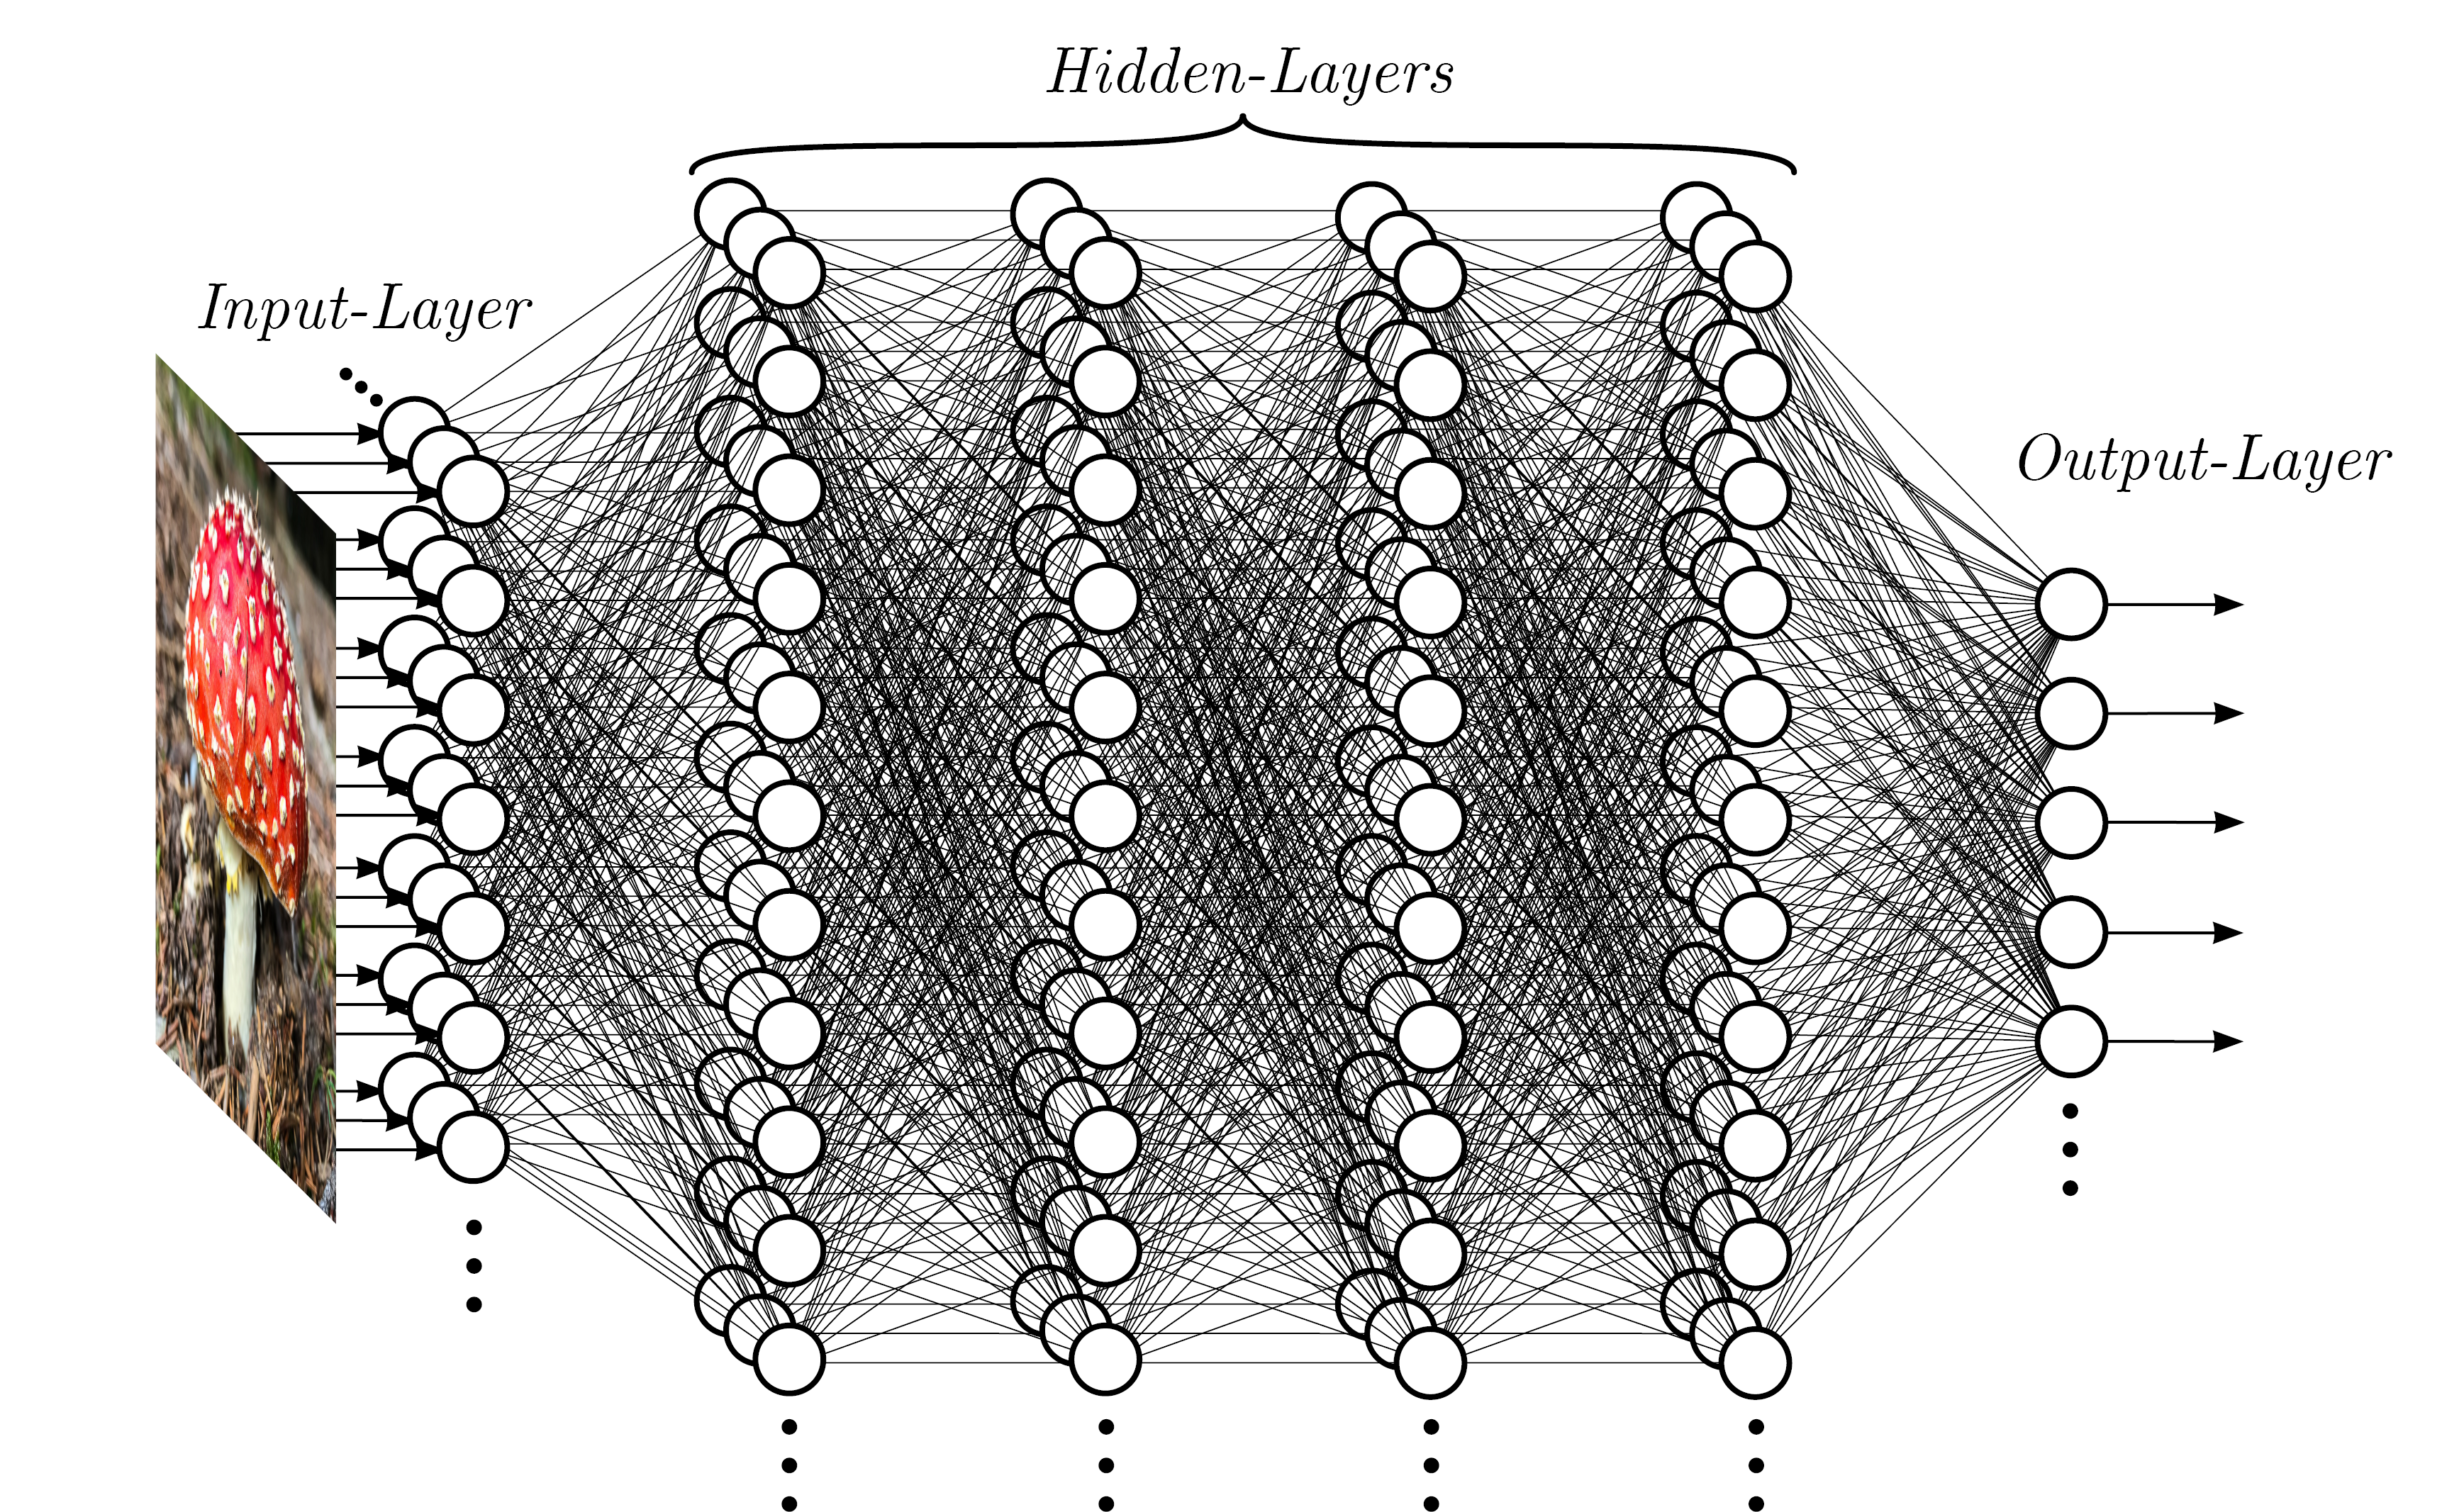
\includegraphics[width=\textwidth]{deep_full_planes}
	\caption[\textit{Fully Connected Deep Neural Network}]{Schema von einem \textit{Fully Connected Deep Neural Network}}
	\label{img:deep_full}
\end{figure}

Per Definition handelt es sich dabei um ein \textit{DNN}, jedoch wird man feststellen, dass sich die Leistung trotz viel langsameren Training nur marginal verbessert. Der Grund dafür liegt in der Mathematik des \textit{Gradient Descent}-Trainingsverfahrens selber: Während dem Training sind Gradienten für \textit{Parameter} der ersten Layers entweder verschwindend klein oder extrem gross, welches das Training destabilisieren. Man nennt dieses Phänomen \textit{Unstable Gradients}. Um das Problem zu umgehen, werden die \textit{Hidden-Layers} in \textit{DNN}s vereinfacht und spezialisiert, um die Anzahl der Verbindungen und somit die der \textit{Parameter} zu verringern. \\

In der Praxis gibt es einige verbreitete \textit{DNN}-Typen: \textit{RNN}s (\textit{Recurrent Neural Networks}), \textit{LSTM RNNs} (\textit{Long short-Term Memory RNN}), \textit{Deep Belief Networks}, etc., jedoch ist das \textit{Convolutional Neural Network} (\textit{CNN}) der geeignetste Typ für Bilderkennungsprobleme. Da es in der Arbeit Pilze anhand von Bildern zu kategorisieren gilt, wird im nächsten Kapitel der Fokus nur auf \textit{CNN}s gelegt.

\subsection{Convolutional Neural Networks}\label{cha:theo:cnn}
Will man ein \textit{DNN} für die Erkennung von Bildern verwenden, so ist das in der Abb. \ref{img:deep_full} gezeigte Netz aus mehreren Gründen ungeeignet: Einerseits leidet es u.a. wegen den vielen Verbindungen weiterhin an \textit{Unstable Gradients} und ist daher schwierig zu trainieren, andererseits werden durch \textit{Fully Connected Layers} die räumlichen Zusammenhänge der Eingangs-Pixel komplett ignoriert. \textit{CNN}s verhindern dies mit sog. \textit{Convolution Layers}. Diese verwenden \textit{Local Receptive Fields}, \textit{Shared Parameters} und \textit{Pooling}, um Kanten und Muster in Bildern zu erkennen.


\subsubsection{Convolution Layer}
Das \textit{Local Receptive Field}, zu Deutsch ''lokales rezeptives Feld'', engt die Eingangssignale eines \textit{Neurons} auf einen lokalisierten Bereich des vorhergehenden Layers ein. Hat man z.B. den \textit{Input-Layer} und einen darauf folgenden \textit{Convolution-Layer}, auf die eine \textit{Local-Receptive-Field}-Grösse von $5\times 5$ \textit{Neuronen} angewandt wird, so ist ein \textit{Neuron} des \textit{Convolution-Layers} nur mit einem $5\times 5$ \textit{Neuronen} grossen Bereich des \textit{Input-Layers} verbunden. Für das erste \textit{Neuron} des \textit{Convolution-Layers} wird es folgendermassen aussehen:

\begin{figure}[h]
	\ContinuedFloat*
	\centering
	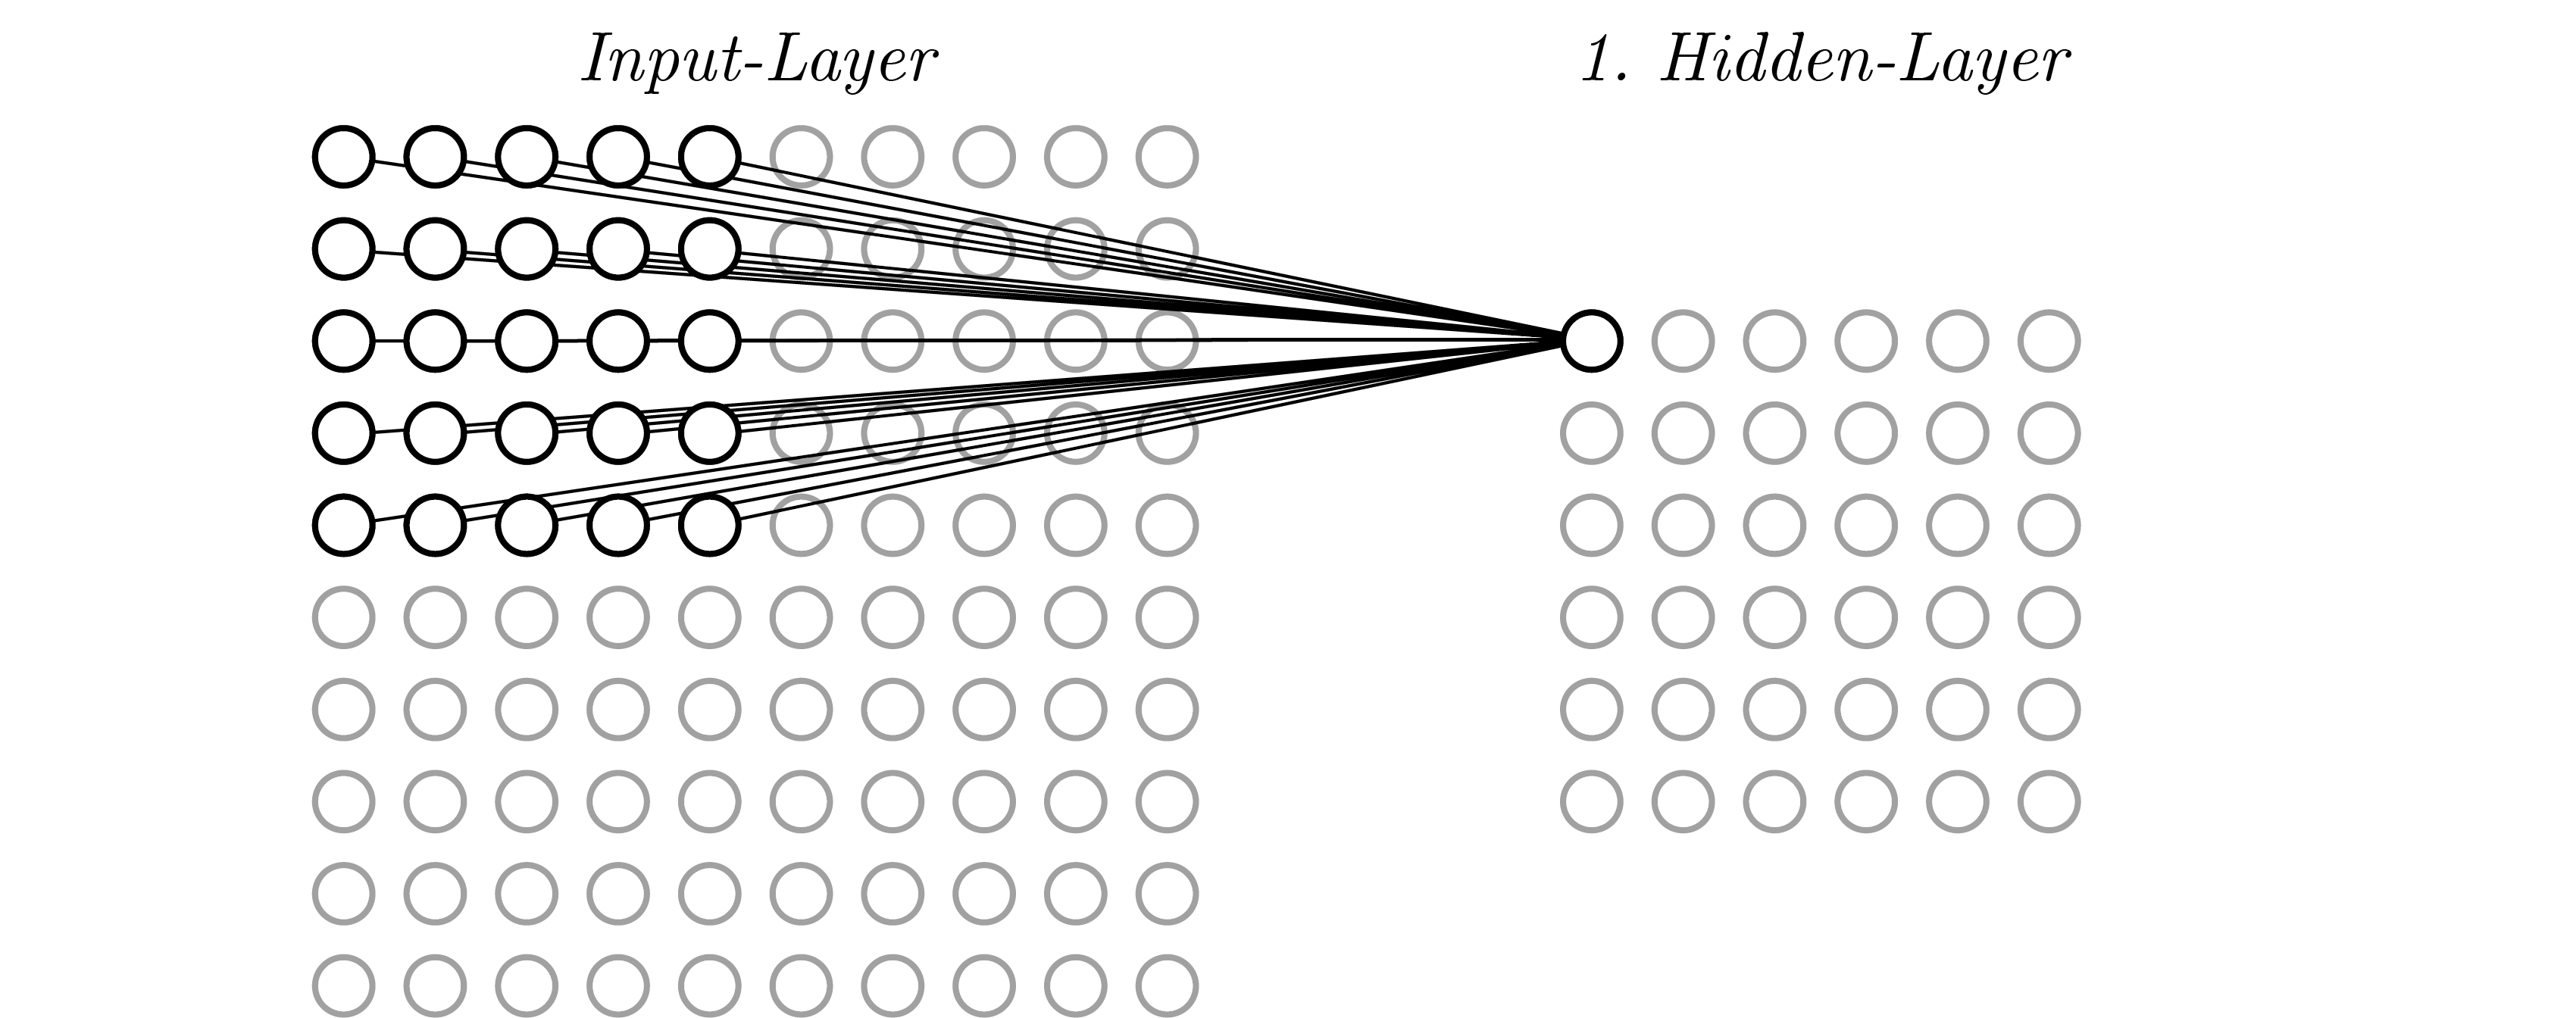
\includegraphics[width=\textwidth]{receptive_field_1}
	\caption[Beispiel für das \textit{Local-Receptive-Field} 1. \textit{Neuron}]{Beispiel für das \textit{Local-Receptive-Field} vom 1. \textit{Neurons} des \textit{Convolution-Layers}}
	\label{img:rec_field1}
\end{figure}

Für das nächste \textit{Neuron} des \textit{Convolution-Layers} verschiebt sich die gesamte Maske einen Schritt in die jeweilige Richtung. Wie die Grösse des \textit{Local-Receptive-Fields} ist auch die Schrittgrösse ein \textit{Meta-Parameter} und kann angepasst werden, in diesem Beispiel wird eine Schrittgrösse von einem \textit{Neuron}(/Pixel) verwendet:

\begin{figure}[h]
	\ContinuedFloat
	\centering
	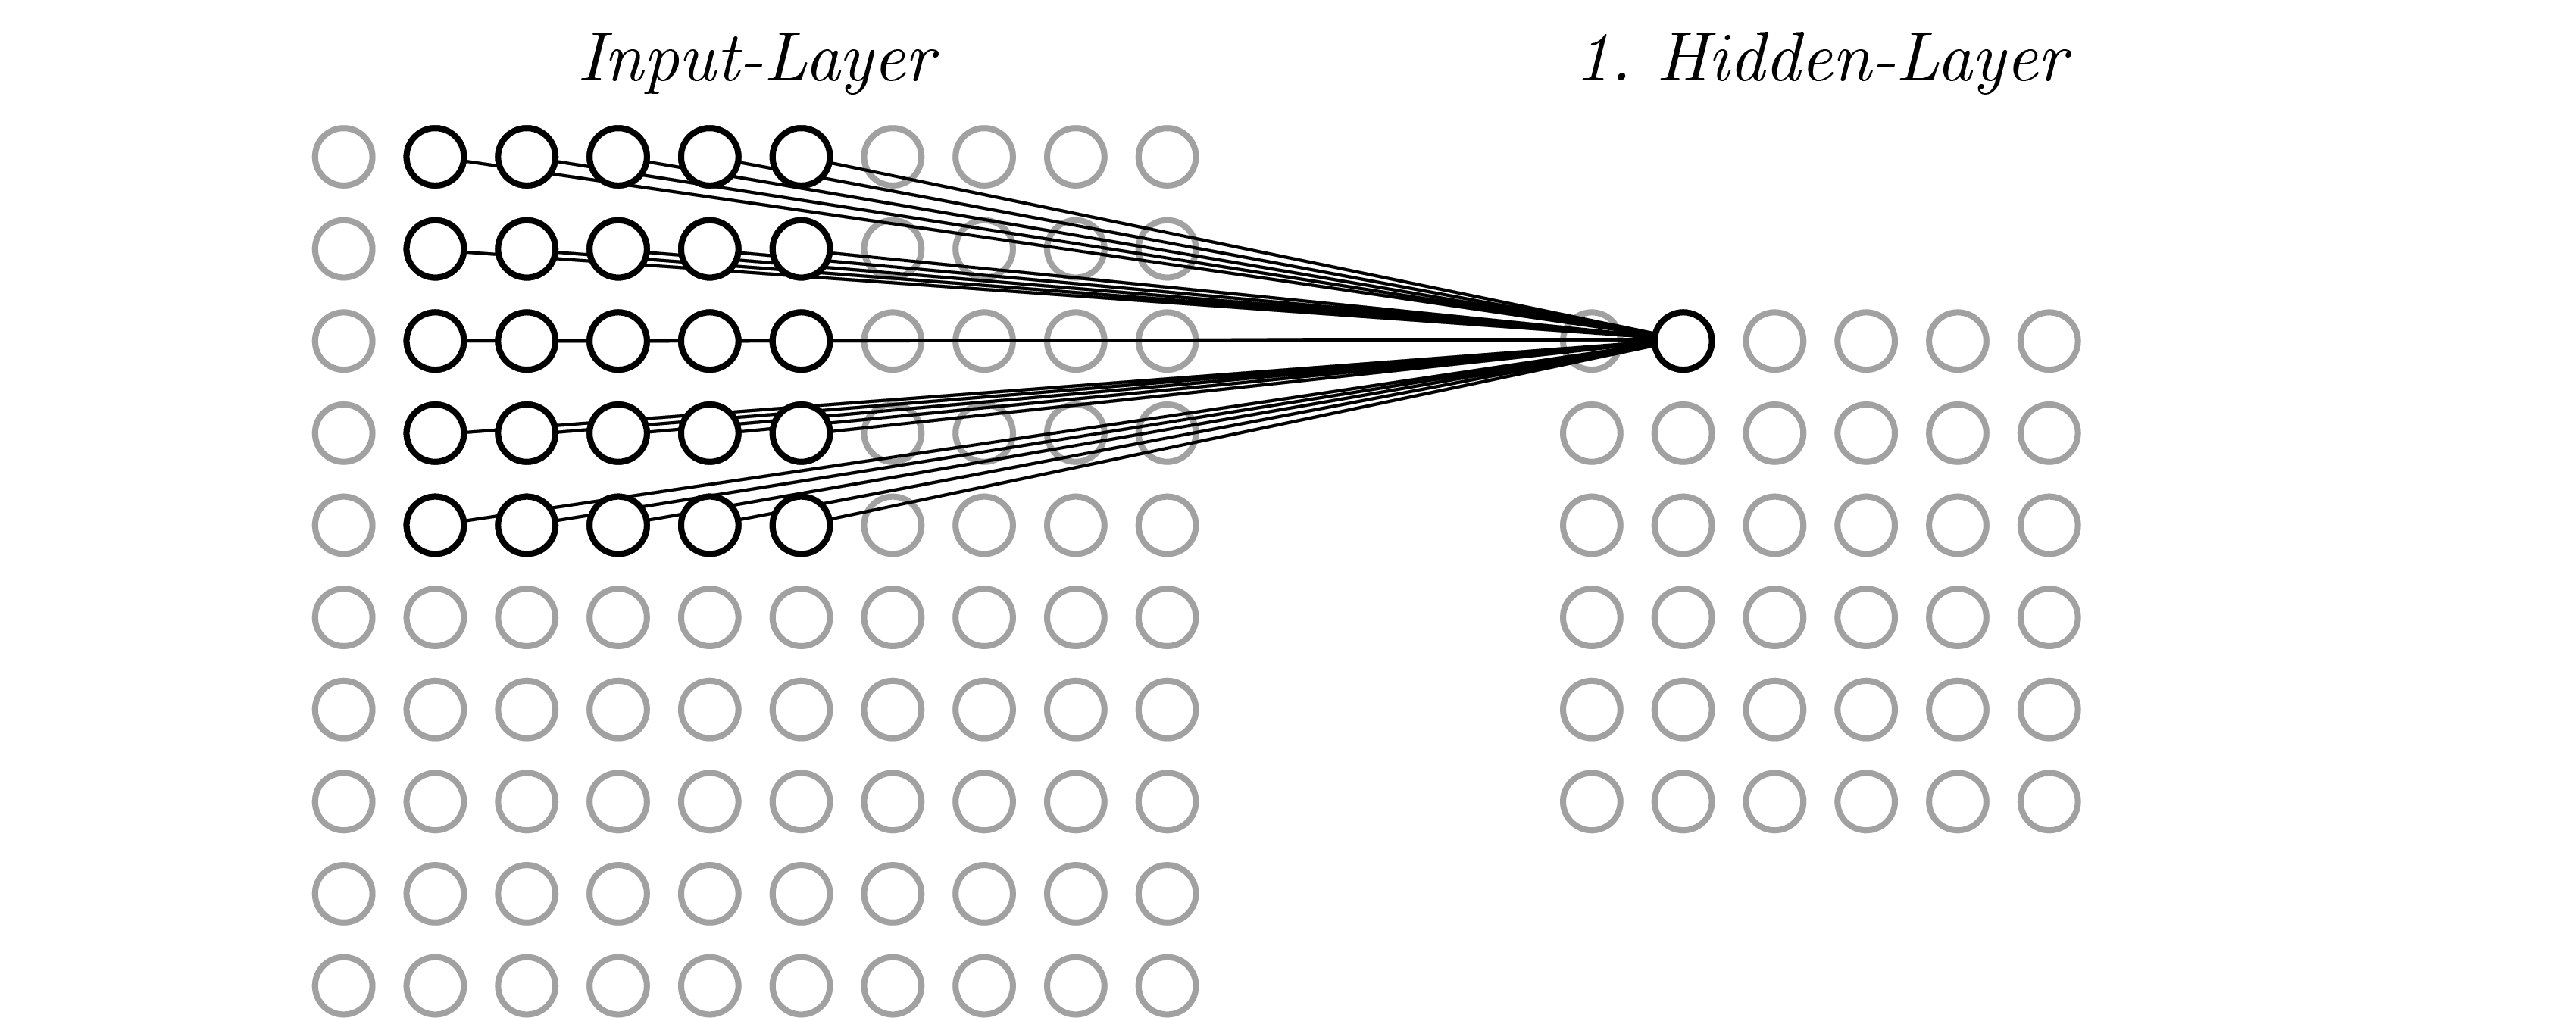
\includegraphics[width=\textwidth]{receptive_field_2}
	\caption[Beispiel für das \textit{Local-Receptive-Field} 2. \textit{Neuron}]{Beispiel für das \textit{Local-Receptive-Field} vom 2. \textit{Neurons} des \textit{Convolution-Layers}}
	\label{img:rec_field2}
\end{figure}

\subsubsection{Feature Maps}
Ein weiterer verwendeter Trick ist, dass alle Neuronen des \textit{Convolution-Layers} dieselben \textit{Parameter} verwenden. Dabei ist die Rede von sog. \textit{Shared weigths}, d.h. das \textit{Neuron}$_{ij}$ im jeweiligen \textit{Local-Receptive-Field} wird für jedes \textit{Convolution-Neuron} mit $w_{ij}$ gewichtet, wobei $i$ und $j$ die Indexes für die horizontale resp. vertikale Position im \textit{Local-Receptive-Field} bezeichnet. Im $5\times 5$-Beispiel von oben gibt es somit nur 25 verschiedene Gewichtungen, der Schwellenwert $b$ ist überall der selbe.

Intuitiv kann man sich den \textit{Convolution Layer} als Schablone für das durch die \textit{Parameter} eingestellte Muster vorstellen, welche Schrittweise über das Eingangsbild geschoben wird. Entspricht das Bild dem Muster, wird ein hoher Wert zurückgegeben und vice versa. Je nach \textit{Parameter} kann man z.B. Kanten oder Ecken erkennen. Man hat somit eine sog. \textit{Feature Map} erstellt, welches das Vorkommen eines bestimmtes Musters im Bild kartiert. Da ein Bild nicht nur aus einem einzigen Muster besteht, werden in einem \textit{Convolution-Layer} sogleich mehrere \textit{Feature-Maps} erstellt, welche sich auf verschiedene Muster spezialisieren können.

\begin{figure}[h]
	\centering
	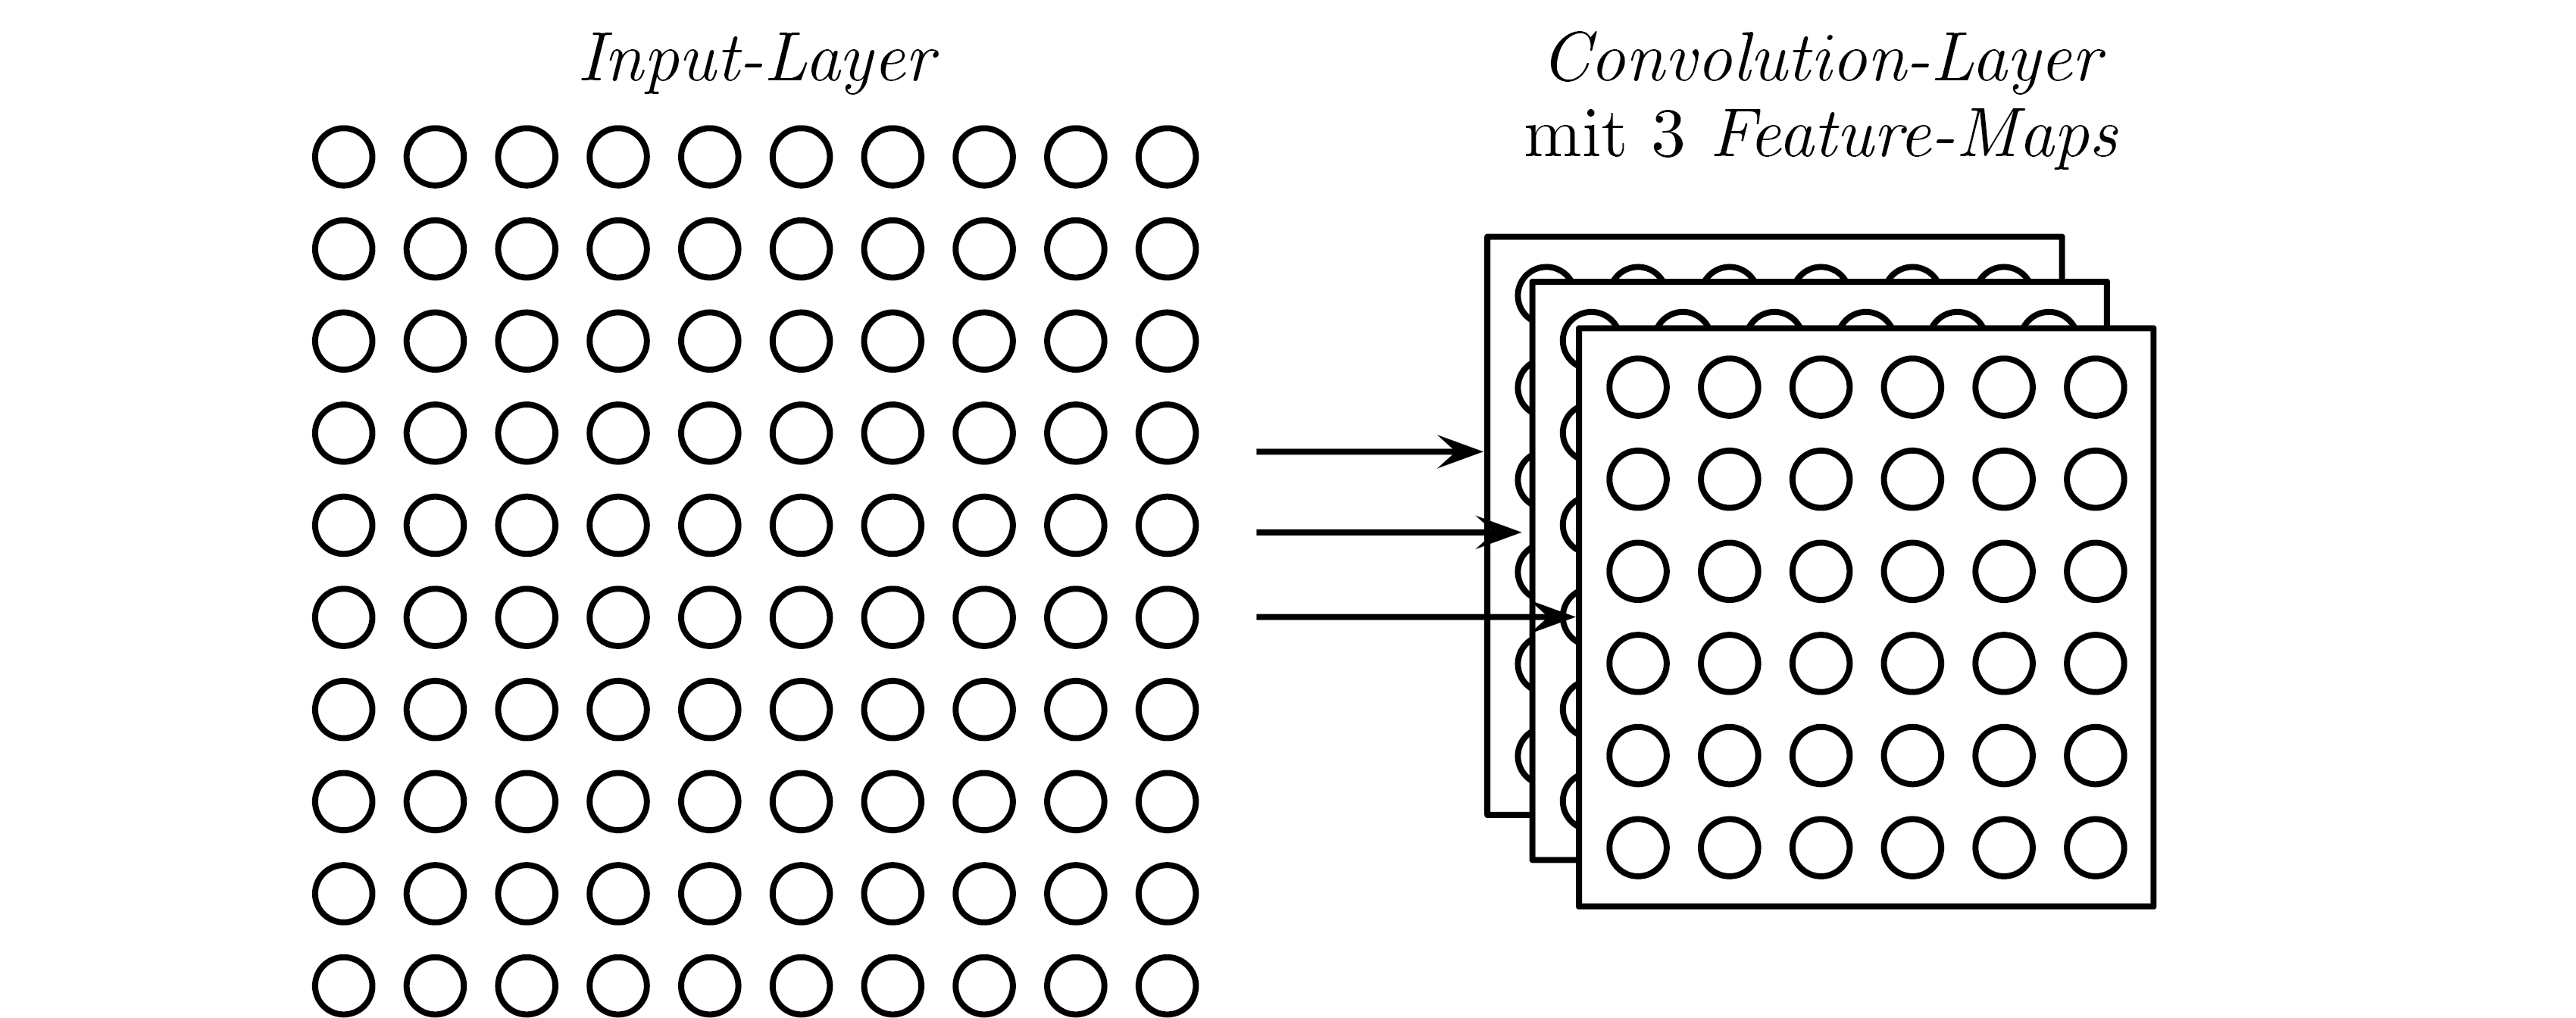
\includegraphics[width=\textwidth]{feature_maps}
	\caption[\textit{Feature-Maps}]{Veranschaulichung von \textit{Feature-Maps}}
	\label{img:feature_maps}
\end{figure}

\subsubsection{Pooling}
Um die vom \textit{Convolution-Layer} erhaltenen \textit{Feature-Maps} weiter zu konzentrieren, folgt in der Regel ein sog. \textit{Pooling}-Layer. Dabei wird wiederum aus einem Bereich des vorherigen \textit{Layers} nur der höchste Wert (\textit{max-Pooling}) oder der durchschnittliche Wert (average-Pooling) an den nächsten \textit{Layer} weitergegeben.

\begin{figure}[h]
	\centering
	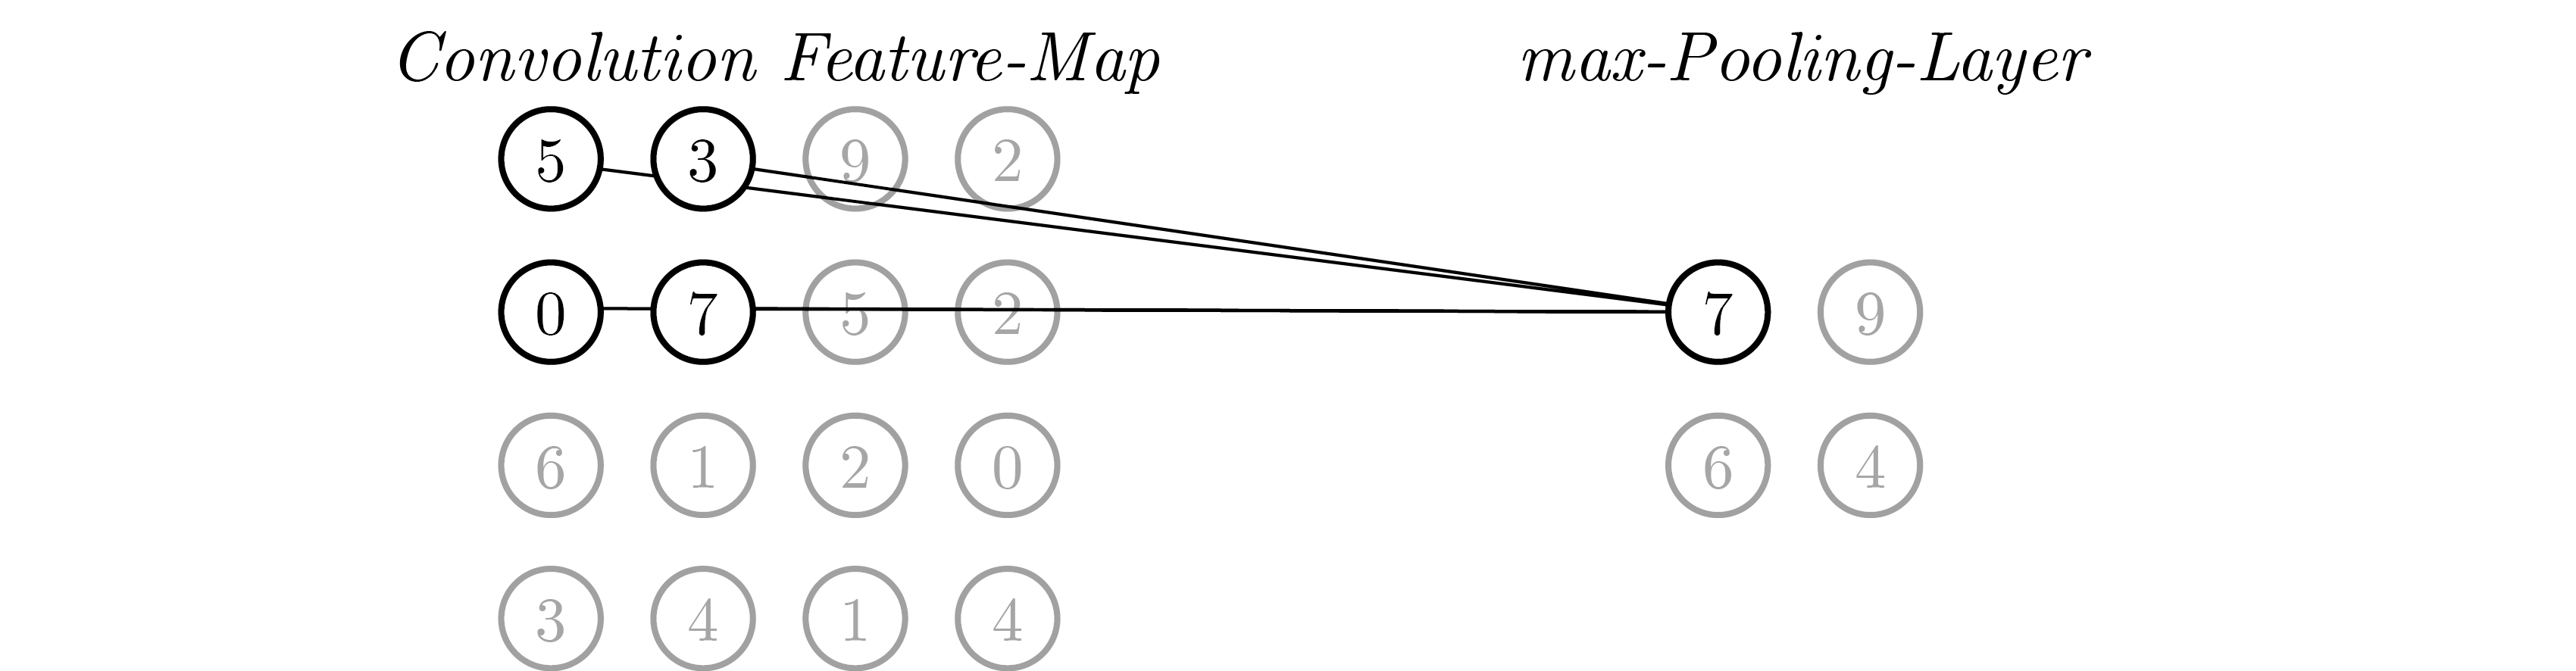
\includegraphics[width=\textwidth]{max_pooling}
	\caption[\textit{\textit{max-Pooling-Layer}}]{Funktionsweise eines \textit{max-Pooling-Layers} mit Filtergrösse $2\times 2$ und Schrittgrösse 2}
	\label{img:max_pooling}
\end{figure}


\subsubsection{Training von \textit{CNN}s}

\subsection{Zusätzliche Meta-Parameter und Modifikation}
Die in den vorherigen Kapiteln beschriebenen \textit{KNN}s und \textit{DNN}s als auch deren Training sind keineswegs starr und lassen sich in vielen Aspekten modifizieren und justieren. Auch diese \textit{Meta-Parameter} sind für spätere Kapitel relevant, weswegen sie in diesem Abschnitt kurz beschrieben werden. 

\subsubsection{ReLU-Layer}
Die \textit{Sigmoid}-Kurve aus Kapitel \ref{cha:theo:neurons} ist nicht die einzige Funktion, die zur Standardisierung des gewichteten Ausgangssignals $z$ eines Neurons (siehe Formel \ref{eq:def_z}) verwendet wird. Neben der \textit{Sigmoid}-Funktion haben sich auch die sog. \textit{Rectified-Linear}-Funktion bewährt. Ein \textit{Neuron}, welches diese Funktion verwendet, nennt man \textit{Rectified-Linear-Unit} (kurz \textit{ReLU}); ein \textit{ReLU}-Layer ist somit eine Schicht zusammengesetzt aus diesen \textit{ReLU}-\textit{Neuronen}.

Im Gegensatz zur \textit{Sigmoid}-Kurve liefert diese Funktion einen ganz anderen Ansatz: Bei $z > 0$ verhält sie sich linear und bei $z \leq 0$ gibt sie einen konstanten Wert von 0 zurück, d.h. der Ausgangswert ist nach oben nicht begrenzt und immer positiv.

\begin{equation}\label{eq:relu_func}
	\sigma(z) = \begin{cases} z, & \mbox{wenn } z > 0 \\ 0, & \mbox{wenn } z \leq 0 \end{cases}
\end{equation}

Als Graph sieht die in der Formel \ref{eq:relu_func} beschriebene \textit{Rectified-Linear}-Funktion verglichen mit der \textit{Sigmoid}-Funktion folgendermassen aus:

\begin{figure}[h]
	\centering
	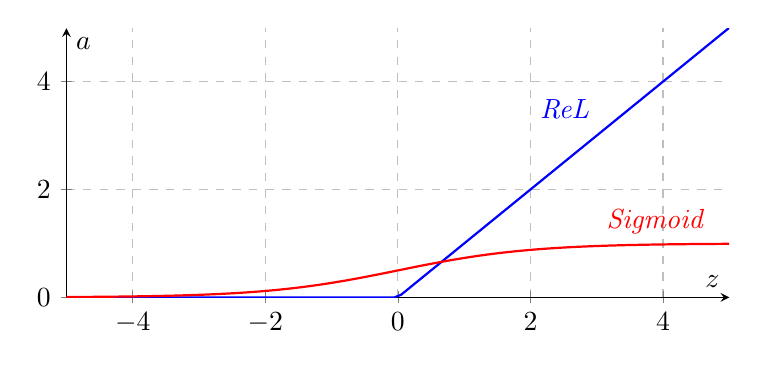
\begin{tikzpicture}
	\begin{axis}[xlabel={$z$},ylabel={$a$},xmin=-5, xmax=5,ymin=0, ymax=4.99,ymajorgrids=true,
	xmajorgrids=true,grid style=dashed,width=10cm,height=5cm,axis line style = <->,
	axis lines=middle,axis y line=left]
	\addplot[-, thick, blue] expression[domain=-5:5,samples=100]{max(0,x)}; 
	\addplot[-, thick, red] expression[domain=-5:5,samples=100]{(1+(2.7182818^(-x)))^(-1)}; 
	\node [right, blue] at (axis cs: 2,3.5) {\textit{ReL}};
	\node [right, red] at (axis cs: 3,1.4) {\textit{Sigmoid}};
	\end{axis}
	\end{tikzpicture}
	\caption[\textit{Rectified-Linear}-Funktion]{\textit{Rectified-Linear}-Funktion $\sigma(z) = max(z,0)$ verglichen mit der \textit{Sigmoid}-Funktion}
	\label{plt:rect_lin}
\end{figure}

\textbf{Vorteile:} Aufgrund der Linearität kann auch für sehr grosse positive $z$-Werte eine signifikante Steigung für die Justierung der \textit{Parameter} berechnet werden, wo hingegen die \textit{Sigmoid}-Funktion in diesem Bereich nur eine verschwindend kleine Steigung liefert. Für negative Werte ist die Steigung hingegen konstant 0, wodurch die \textit{Parameter} jenes Neurons nicht mehr durch das Training justiert werden können und gewissermassen ''einfrieren''. Diese Massnahme kann in machen Anwendungsszenarien die Leistung des \textit{KNN}s verbessern.

\subsubsection{Fehlerberechnung}
Anstelle der \textit{Quadratic Cost}-Funktion aus Kapitel \ref{cha:theo:cost} zur Berechnung des Fehlers \textit{Err}, kann auch die \textit{Cross-Entropy-Cost}-Funktion verwendet werden:

\begin{equation}\label{eq:cross_enropy_cost}
C(A_1,...,A_m,y_1,...,y_m)=-\sum_{i=1}^{m}\left[ y_i \cdot ln(a) + (1-y_i)\cdot ln(1-A_i)\right]
\end{equation}

Diese \textit{Cost}-Funktion kann grosse Fehlerwerte für \textit{Sigmoid-Neuronen} besser handhaben, welche bei der \textit{Quadratic Cost}-Funktion z.T. zu einer Verlangsamung des Trainingsprozesses führen können.

\subsubsection{Dropout-Layer}

\subsubsection{Data Augmentation}

\subsubsection{Transfer Learning}

\subsubsection{Ensemble}




















%\begin{figure}[ht]
%	\centering
%	\begin{tikzpicture}
%	\begin{axis}[xlabel={$p$},	ylabel={$Err$},	xmin=-0, xmax=9.9,	ymin=0, ymax=4.999,	ymajorgrids=true,	xmajorgrids=true,	grid style=dashed,	width=10cm,	height=5cm,
%	axis line style = <->,	axis lines=middle,	axis x line=bottom,	axis y line=left
%	]
%	\addplot[-, thick, blue] expression[domain=0:10,samples=100]{-0.0026*x^5+0.0641*x^4-0.5233*x^3+1.6965*x^2-2.5210*x+4.5000};

%	\node[anchor=center] (source) at (axis cs:3,4){};
%	\node (destination) at (axis cs:3,2.7){};
%	\draw[->, thick, red](source)--(destination);

%	\end{axis}
%	\end{tikzpicture}
%	\caption[Sigmoid-Funktion]{Beispiel: Fehler $Err$ als Funktion eines \textit{Parameters} $p$}
%	\label{plt:paraboloid}
%\end{figure}


%\begin{equation}\label{eq:part_der}
%\Delta a \approx \sum_{i=1}^{n} \frac{\delta a}{\delta w_i}\Delta w_j + \frac{\delta a}{\delta b}\Delta b
%\end{equation}